% Options for packages loaded elsewhere
\PassOptionsToPackage{unicode}{hyperref}
\PassOptionsToPackage{hyphens}{url}
%
\documentclass[
]{article}
\usepackage{amsmath,amssymb}
\usepackage{lmodern}
\usepackage{iftex}
\ifPDFTeX
  \usepackage[T1]{fontenc}
  \usepackage[utf8]{inputenc}
  \usepackage{textcomp} % provide euro and other symbols
\else % if luatex or xetex
  \usepackage{unicode-math}
  \defaultfontfeatures{Scale=MatchLowercase}
  \defaultfontfeatures[\rmfamily]{Ligatures=TeX,Scale=1}
\fi
% Use upquote if available, for straight quotes in verbatim environments
\IfFileExists{upquote.sty}{\usepackage{upquote}}{}
\IfFileExists{microtype.sty}{% use microtype if available
  \usepackage[]{microtype}
  \UseMicrotypeSet[protrusion]{basicmath} % disable protrusion for tt fonts
}{}
\makeatletter
\@ifundefined{KOMAClassName}{% if non-KOMA class
  \IfFileExists{parskip.sty}{%
    \usepackage{parskip}
  }{% else
    \setlength{\parindent}{0pt}
    \setlength{\parskip}{6pt plus 2pt minus 1pt}}
}{% if KOMA class
  \KOMAoptions{parskip=half}}
\makeatother
\usepackage{xcolor}
\IfFileExists{xurl.sty}{\usepackage{xurl}}{} % add URL line breaks if available
\IfFileExists{bookmark.sty}{\usepackage{bookmark}}{\usepackage{hyperref}}
\hypersetup{
  pdftitle={病历本},
  pdfauthor={Yiyi},
  hidelinks,
  pdfcreator={LaTeX via pandoc}}
\urlstyle{same} % disable monospaced font for URLs
\usepackage[margin=1in]{geometry}
\usepackage{color}
\usepackage{fancyvrb}
\newcommand{\VerbBar}{|}
\newcommand{\VERB}{\Verb[commandchars=\\\{\}]}
\DefineVerbatimEnvironment{Highlighting}{Verbatim}{commandchars=\\\{\}}
% Add ',fontsize=\small' for more characters per line
\usepackage{framed}
\definecolor{shadecolor}{RGB}{248,248,248}
\newenvironment{Shaded}{\begin{snugshade}}{\end{snugshade}}
\newcommand{\AlertTok}[1]{\textcolor[rgb]{0.94,0.16,0.16}{#1}}
\newcommand{\AnnotationTok}[1]{\textcolor[rgb]{0.56,0.35,0.01}{\textbf{\textit{#1}}}}
\newcommand{\AttributeTok}[1]{\textcolor[rgb]{0.77,0.63,0.00}{#1}}
\newcommand{\BaseNTok}[1]{\textcolor[rgb]{0.00,0.00,0.81}{#1}}
\newcommand{\BuiltInTok}[1]{#1}
\newcommand{\CharTok}[1]{\textcolor[rgb]{0.31,0.60,0.02}{#1}}
\newcommand{\CommentTok}[1]{\textcolor[rgb]{0.56,0.35,0.01}{\textit{#1}}}
\newcommand{\CommentVarTok}[1]{\textcolor[rgb]{0.56,0.35,0.01}{\textbf{\textit{#1}}}}
\newcommand{\ConstantTok}[1]{\textcolor[rgb]{0.00,0.00,0.00}{#1}}
\newcommand{\ControlFlowTok}[1]{\textcolor[rgb]{0.13,0.29,0.53}{\textbf{#1}}}
\newcommand{\DataTypeTok}[1]{\textcolor[rgb]{0.13,0.29,0.53}{#1}}
\newcommand{\DecValTok}[1]{\textcolor[rgb]{0.00,0.00,0.81}{#1}}
\newcommand{\DocumentationTok}[1]{\textcolor[rgb]{0.56,0.35,0.01}{\textbf{\textit{#1}}}}
\newcommand{\ErrorTok}[1]{\textcolor[rgb]{0.64,0.00,0.00}{\textbf{#1}}}
\newcommand{\ExtensionTok}[1]{#1}
\newcommand{\FloatTok}[1]{\textcolor[rgb]{0.00,0.00,0.81}{#1}}
\newcommand{\FunctionTok}[1]{\textcolor[rgb]{0.00,0.00,0.00}{#1}}
\newcommand{\ImportTok}[1]{#1}
\newcommand{\InformationTok}[1]{\textcolor[rgb]{0.56,0.35,0.01}{\textbf{\textit{#1}}}}
\newcommand{\KeywordTok}[1]{\textcolor[rgb]{0.13,0.29,0.53}{\textbf{#1}}}
\newcommand{\NormalTok}[1]{#1}
\newcommand{\OperatorTok}[1]{\textcolor[rgb]{0.81,0.36,0.00}{\textbf{#1}}}
\newcommand{\OtherTok}[1]{\textcolor[rgb]{0.56,0.35,0.01}{#1}}
\newcommand{\PreprocessorTok}[1]{\textcolor[rgb]{0.56,0.35,0.01}{\textit{#1}}}
\newcommand{\RegionMarkerTok}[1]{#1}
\newcommand{\SpecialCharTok}[1]{\textcolor[rgb]{0.00,0.00,0.00}{#1}}
\newcommand{\SpecialStringTok}[1]{\textcolor[rgb]{0.31,0.60,0.02}{#1}}
\newcommand{\StringTok}[1]{\textcolor[rgb]{0.31,0.60,0.02}{#1}}
\newcommand{\VariableTok}[1]{\textcolor[rgb]{0.00,0.00,0.00}{#1}}
\newcommand{\VerbatimStringTok}[1]{\textcolor[rgb]{0.31,0.60,0.02}{#1}}
\newcommand{\WarningTok}[1]{\textcolor[rgb]{0.56,0.35,0.01}{\textbf{\textit{#1}}}}
\usepackage{longtable,booktabs,array}
\usepackage{calc} % for calculating minipage widths
% Correct order of tables after \paragraph or \subparagraph
\usepackage{etoolbox}
\makeatletter
\patchcmd\longtable{\par}{\if@noskipsec\mbox{}\fi\par}{}{}
\makeatother
% Allow footnotes in longtable head/foot
\IfFileExists{footnotehyper.sty}{\usepackage{footnotehyper}}{\usepackage{footnote}}
\makesavenoteenv{longtable}
\usepackage{graphicx}
\makeatletter
\def\maxwidth{\ifdim\Gin@nat@width>\linewidth\linewidth\else\Gin@nat@width\fi}
\def\maxheight{\ifdim\Gin@nat@height>\textheight\textheight\else\Gin@nat@height\fi}
\makeatother
% Scale images if necessary, so that they will not overflow the page
% margins by default, and it is still possible to overwrite the defaults
% using explicit options in \includegraphics[width, height, ...]{}
\setkeys{Gin}{width=\maxwidth,height=\maxheight,keepaspectratio}
% Set default figure placement to htbp
\makeatletter
\def\fps@figure{htbp}
\makeatother
\setlength{\emergencystretch}{3em} % prevent overfull lines
\providecommand{\tightlist}{%
  \setlength{\itemsep}{0pt}\setlength{\parskip}{0pt}}
\setcounter{secnumdepth}{-\maxdimen} % remove section numbering
\ifLuaTeX
  \usepackage{selnolig}  % disable illegal ligatures
\fi

\title{病历本}
\author{Yiyi}
\date{2021-08-04}

\begin{document}
\maketitle

{
\setcounter{tocdepth}{3}
\tableofcontents
}
\hypertarget{section}{%
\section{}\label{section}}

\begin{Shaded}
\begin{Highlighting}[]
 \FunctionTok{rm}\NormalTok{(}\AttributeTok{list =} \FunctionTok{ls}\NormalTok{())}
\end{Highlighting}
\end{Shaded}

\hypertarget{packages}{%
\subsection{Packages}\label{packages}}

lag 是2:13 代表1:12. newdata里的1代表的是原数据. 首先把2:13 存储起来,
用paste0(2:13,加上''\$``)用来匹配以2:13数字结尾的列?

\begin{Shaded}
\begin{Highlighting}[]
\FunctionTok{select}\NormalTok{(x,}\FunctionTok{starts\_with}\NormalTok{(}\StringTok{"s"}\NormalTok{)) or }\FunctionTok{select}\NormalTok{(df,}\FunctionTok{end\_with}\NormalTok{(}\StringTok{"string"}\NormalTok{)) 句法 等同于df}\SpecialCharTok{\%\textgreater{}\%}\FunctionTok{select}\NormalTok{(}\FunctionTok{matches}\NormalTok{(}\StringTok{"$"}\NormalTok{))}
\end{Highlighting}
\end{Shaded}

这两种做法都和之前是完全相等. 都只针对\textbf{列}操作,对表格内容无关.
在此只保留

\begin{Shaded}
\begin{Highlighting}[]
\FunctionTok{select}\NormalTok{(df,}\FunctionTok{end\_with}\NormalTok{(}\StringTok{"s"}\NormalTok{))}
\end{Highlighting}
\end{Shaded}

后续可以查看git 完全匹配字段的两种算法 commit

\hypertarget{lag-and-vat}{%
\subsection{Lag and VAT}\label{lag-and-vat}}

\begin{Shaded}
\begin{Highlighting}[]
\NormalTok{old13}\OtherTok{\textless{}{-}}\FunctionTok{c}\NormalTok{(}\DecValTok{2}\SpecialCharTok{:}\DecValTok{13}\NormalTok{)}
\ControlFlowTok{for}\NormalTok{ (i }\ControlFlowTok{in} \DecValTok{1}\SpecialCharTok{:}\DecValTok{12}\NormalTok{) \{}

  \FunctionTok{assign}\NormalTok{(}\FunctionTok{paste0}\NormalTok{(}\StringTok{"lag"}\NormalTok{,i),}\FunctionTok{select}\NormalTok{(newdata,}\FunctionTok{ends\_with}\NormalTok{(}\FunctionTok{paste0}\NormalTok{(old13[i]))))}

\NormalTok{\}}
\NormalTok{lag1 }\OtherTok{\textless{}{-}}\NormalTok{ lag1 }\SpecialCharTok{\%\textgreater{}\%} \FunctionTok{select}\NormalTok{(}\SpecialCharTok{{-}}\FunctionTok{contains}\NormalTok{(}\StringTok{"12"}\NormalTok{))}
\NormalTok{lag2 }\OtherTok{\textless{}{-}}\NormalTok{ lag2 }\SpecialCharTok{\%\textgreater{}\%} \FunctionTok{select}\NormalTok{(}\SpecialCharTok{{-}}\FunctionTok{contains}\NormalTok{(}\StringTok{"13"}\NormalTok{))}
\NormalTok{VAT1 }\OtherTok{\textless{}{-}} \FunctionTok{as.numeric}\NormalTok{(newdata}\SpecialCharTok{$}\StringTok{\textasciigrave{}}\AttributeTok{time1}\StringTok{\textasciigrave{}} \SpecialCharTok{==} \StringTok{"2008{-}12{-}01"}\NormalTok{)}
\NormalTok{VAT2 }\OtherTok{\textless{}{-}} \FunctionTok{as.numeric}\NormalTok{(newdata}\SpecialCharTok{$}\StringTok{\textasciigrave{}}\AttributeTok{time1}\StringTok{\textasciigrave{}} \SpecialCharTok{==} \StringTok{"2010{-}01{-}01"}\NormalTok{)}
\NormalTok{VAT3 }\OtherTok{\textless{}{-}} \FunctionTok{as.numeric}\NormalTok{(newdata}\SpecialCharTok{$}\StringTok{\textasciigrave{}}\AttributeTok{time1}\StringTok{\textasciigrave{}} \SpecialCharTok{==} \StringTok{"2011{-}01{-}01"}\NormalTok{)}
\NormalTok{Recession }\OtherTok{\textless{}{-}} \FunctionTok{as.numeric}\NormalTok{(newdata}\SpecialCharTok{$}\StringTok{\textasciigrave{}}\AttributeTok{time1}\StringTok{\textasciigrave{}} \SpecialCharTok{\textgreater{}=} \StringTok{"2008{-}04{-}01"} \SpecialCharTok{\&}\NormalTok{ newdata}\SpecialCharTok{$}\StringTok{\textasciigrave{}}\AttributeTok{time1}\StringTok{\textasciigrave{}}\SpecialCharTok{\textless{}=} \StringTok{"2009{-}06{-}01"}\NormalTok{)}
\end{Highlighting}
\end{Shaded}

\hypertarget{monthly-dummies-variable-position}{%
\subsection{Monthly dummies variable
position}\label{monthly-dummies-variable-position}}

\begin{Shaded}
\begin{Highlighting}[]
\NormalTok{monthname}\OtherTok{\textless{}{-}}\FunctionTok{c}\NormalTok{(}\StringTok{"time\_Apr"}\NormalTok{,}\StringTok{"time\_Aug"}\NormalTok{, }\StringTok{"time\_Dec"}\NormalTok{,  }\StringTok{"time\_Jan"}\NormalTok{,}\StringTok{"time\_Jul"}\NormalTok{,}\StringTok{"time\_Jun"}\NormalTok{ ,}\StringTok{"time\_Mar"}\NormalTok{,}\StringTok{"time\_May"}\NormalTok{,}\StringTok{"time\_Nov"}\NormalTok{,}\StringTok{"time\_Oct"}\NormalTok{,}\StringTok{"time\_Sep"}\NormalTok{)}

\ControlFlowTok{for}\NormalTok{ (i }\ControlFlowTok{in} \DecValTok{1}\SpecialCharTok{:}\FunctionTok{length}\NormalTok{(monthname)) \{}
  \FunctionTok{print}\NormalTok{(}
 \FunctionTok{which}\NormalTok{(}\FunctionTok{colnames}\NormalTok{(newdata)}\SpecialCharTok{==}\NormalTok{monthname[i])}
\NormalTok{)}
\NormalTok{\}}
\end{Highlighting}
\end{Shaded}

\begin{verbatim}
## [1] 2251
## [1] 2252
## [1] 2253
## [1] 2254
## [1] 2255
## [1] 2256
## [1] 2257
## [1] 2258
## [1] 2259
## [1] 2260
## [1] 2261
\end{verbatim}

\hypertarget{create-time_apr-etc.}{%
\subsection{Create time\_Apr etc.}\label{create-time_apr-etc.}}

the correct version. 首先把月度虚拟变量存储到cpilag 里.
然后用同一迭代变量 送到各自的time\_下. \textbf{注意,
双迭代变量还未完全掌握, i 和j 一起用 必出错}

\begin{Shaded}
\begin{Highlighting}[]
\NormalTok{monthdummies}\OtherTok{\textless{}{-}}\NormalTok{newdata[,}\DecValTok{2251}\SpecialCharTok{:}\DecValTok{2261}\NormalTok{]}

  \ControlFlowTok{for}\NormalTok{ (i }\ControlFlowTok{in} \DecValTok{1}\SpecialCharTok{:}\DecValTok{11}\NormalTok{) \{}
  \FunctionTok{assign}\NormalTok{(}\FunctionTok{colnames}\NormalTok{(monthdummies)[i],}\FunctionTok{as.numeric}\NormalTok{(}\FunctionTok{unlist}\NormalTok{(monthdummies[[i]])))}
\NormalTok{  \}}
\end{Highlighting}
\end{Shaded}

\hypertarget{cpi-ldv-variables-position}{%
\subsection{CPI LDV variables
position}\label{cpi-ldv-variables-position}}

\begin{Shaded}
\begin{Highlighting}[]
\NormalTok{lag.list }\OtherTok{\textless{}{-}} \FunctionTok{mget}\NormalTok{(}\FunctionTok{paste0}\NormalTok{(}\StringTok{"lag"}\NormalTok{, }\DecValTok{1}\SpecialCharTok{:}\DecValTok{12}\NormalTok{))}


\ControlFlowTok{for}\NormalTok{ (i }\ControlFlowTok{in} \DecValTok{1}\SpecialCharTok{:}\DecValTok{12}\NormalTok{) \{}
  \FunctionTok{assign}\NormalTok{(}\FunctionTok{paste0}\NormalTok{(}\StringTok{"lag"}\NormalTok{,i),}\FunctionTok{as.data.frame}\NormalTok{(lag.list[[i]]))}
\NormalTok{\}}

\NormalTok{COPY }\OtherTok{\textless{}{-}} \FunctionTok{as.data.frame}\NormalTok{(COPY)}



\CommentTok{\# CPI{-}LAGS {-}{-}{-}{-}{-}{-}{-}{-}{-}{-}{-}{-}{-}{-}{-}{-}{-}{-}{-}{-}{-}{-}{-}{-}{-}{-}{-}{-}{-}{-}{-}{-}{-}{-}{-}{-}{-}{-}{-}{-}{-}{-}{-}{-}{-}{-}{-}{-}{-}{-}{-}{-}{-}{-}{-}{-}{-}{-}{-}{-}{-}{-}{-}{-}}
\NormalTok{cpi.list}\OtherTok{\textless{}{-}}\FunctionTok{c}\NormalTok{(}\FunctionTok{paste0}\NormalTok{(}\StringTok{"CPI ALL ITEMS"}\NormalTok{,}\DecValTok{2}\SpecialCharTok{:}\DecValTok{13}\NormalTok{))}

\ControlFlowTok{for}\NormalTok{ (i }\ControlFlowTok{in} \DecValTok{1}\SpecialCharTok{:}\FunctionTok{length}\NormalTok{(cpi.list)) \{}
  \FunctionTok{print}\NormalTok{(}\FunctionTok{which}\NormalTok{(}\FunctionTok{colnames}\NormalTok{(newdata)}\SpecialCharTok{==}\NormalTok{cpi.list[i]))}
  
\NormalTok{\}   }
\end{Highlighting}
\end{Shaded}

\begin{verbatim}
## [1] 2
## [1] 3
## [1] 4
## [1] 5
## [1] 6
## [1] 7
## [1] 8
## [1] 9
## [1] 10
## [1] 11
## [1] 12
## [1] 13
\end{verbatim}

\begin{Shaded}
\begin{Highlighting}[]
\NormalTok{cpilag}\OtherTok{\textless{}{-}}\NormalTok{newdata[,}\DecValTok{2}\SpecialCharTok{:}\DecValTok{13}\NormalTok{]}
\ControlFlowTok{for}\NormalTok{ (i }\ControlFlowTok{in} \DecValTok{1}\SpecialCharTok{:}\DecValTok{12}\NormalTok{) \{}

    
 
  \FunctionTok{assign}\NormalTok{(}\FunctionTok{paste0}\NormalTok{(}\StringTok{"CPI\_lag"}\NormalTok{,i),}\FunctionTok{as.numeric}\NormalTok{(}\FunctionTok{unlist}\NormalTok{(cpilag[,..i])))}
  
\NormalTok{\}}
\end{Highlighting}
\end{Shaded}

\hypertarget{rgression}{%
\subsection{Rgression}\label{rgression}}

\begin{Shaded}
\begin{Highlighting}[]
\CommentTok{\# Regression Equation {-}{-}{-}{-}{-}{-}{-}{-}{-}{-}{-}{-}{-}{-}{-}{-}{-}{-}{-}{-}{-}{-}{-}{-}{-}{-}{-}{-}{-}{-}{-}{-}{-}{-}{-}{-}{-}{-}{-}{-}{-}{-}{-}{-}{-}{-}{-}{-}{-}{-}{-}{-}{-}}


\NormalTok{reg.model }\OtherTok{\textless{}{-}} \FunctionTok{lapply}\NormalTok{(}\DecValTok{1}\SpecialCharTok{:}\DecValTok{173}\NormalTok{, }\ControlFlowTok{function}\NormalTok{(x) }\FunctionTok{lm}\NormalTok{(COPY[,x] }\SpecialCharTok{\textasciitilde{}}\NormalTok{ lag1[,x]}\SpecialCharTok{+}\NormalTok{lag2[,x]}\SpecialCharTok{+}\NormalTok{lag3[,x]}\SpecialCharTok{+}\NormalTok{lag4[,x]}\SpecialCharTok{+}
\NormalTok{                                            lag5[,x]}\SpecialCharTok{+}\NormalTok{lag6[,x]}\SpecialCharTok{+}\NormalTok{lag7[,x]}\SpecialCharTok{+}\NormalTok{lag8[,x]}\SpecialCharTok{+}\NormalTok{lag9[,x]}\SpecialCharTok{+}
\NormalTok{                                            lag10[,x]}\SpecialCharTok{+}\NormalTok{lag11[,x]}\SpecialCharTok{+}\NormalTok{lag12[,x]}\SpecialCharTok{+}\NormalTok{ time\_Aug }\SpecialCharTok{+} 
\NormalTok{                                            time\_Dec}\SpecialCharTok{+}\NormalTok{ time\_Apr}\SpecialCharTok{+}\NormalTok{ time\_Jan}\SpecialCharTok{+}\NormalTok{time\_Jul}\SpecialCharTok{+}\NormalTok{time\_Jun }\SpecialCharTok{+}
\NormalTok{                                            time\_Mar}\SpecialCharTok{+}\NormalTok{time\_May}\SpecialCharTok{+}\NormalTok{time\_Nov}\SpecialCharTok{+}\NormalTok{time\_Oct}\SpecialCharTok{+}\NormalTok{time\_Sep}\SpecialCharTok{+}\NormalTok{VAT1}\SpecialCharTok{+}\NormalTok{VAT2}\SpecialCharTok{+}\NormalTok{VAT3}\SpecialCharTok{+}\NormalTok{Recession}\SpecialCharTok{+}\NormalTok{Trend)}
\NormalTok{)}

\ControlFlowTok{for}\NormalTok{ (i }\ControlFlowTok{in} \DecValTok{1}\SpecialCharTok{:}\DecValTok{173}\NormalTok{) \{}
  \FunctionTok{names}\NormalTok{(reg.model[[i]]}\SpecialCharTok{$}\NormalTok{coefficients)}\OtherTok{\textless{}{-}}\FunctionTok{c}\NormalTok{(}\StringTok{\textquotesingle{}Constant\textquotesingle{}}\NormalTok{,}\StringTok{\textquotesingle{}lag1\textquotesingle{}}\NormalTok{,}\StringTok{\textquotesingle{}lag2\textquotesingle{}}\NormalTok{,}\StringTok{"lag3"}\NormalTok{,}\StringTok{"lag4"}\NormalTok{,}\StringTok{"lag5"}\NormalTok{,}\StringTok{"lag6"}\NormalTok{,}\StringTok{"lag7"}\NormalTok{,}\StringTok{"lag8"}\NormalTok{,}\StringTok{"lag9"}\NormalTok{,}\StringTok{"lag10"}\NormalTok{,}\StringTok{"lag11"}\NormalTok{,}\StringTok{"lag12"}\NormalTok{,}
                                        \StringTok{"time\_Aug"}\NormalTok{ , }
                                        \StringTok{"time\_Dec"}\NormalTok{, }\StringTok{"time\_Feb"}\NormalTok{, }\StringTok{"time\_Jan"}\NormalTok{,}\StringTok{"time\_Jul"}\NormalTok{,}\StringTok{"time\_Jun"}\NormalTok{ ,}\StringTok{"time\_Mar"}\NormalTok{,}
                                        \StringTok{"time\_May"}\NormalTok{,}\StringTok{"time\_Nov"}\NormalTok{,}\StringTok{"time\_Oct"}\NormalTok{,}\StringTok{"time\_Sep"}\NormalTok{,}\StringTok{"VAT1"}\NormalTok{,}\StringTok{"VAT2"}\NormalTok{,}\StringTok{"VAT3"}\NormalTok{,}\StringTok{"Recession"}\NormalTok{,}\StringTok{"Trend"}\NormalTok{)}
\NormalTok{\}}

\NormalTok{regression }\OtherTok{\textless{}{-}} \FunctionTok{lapply}\NormalTok{(}\DecValTok{1}\SpecialCharTok{:}\DecValTok{122}\NormalTok{, }\ControlFlowTok{function}\NormalTok{(x) }\FunctionTok{lm}\NormalTok{(COPY[,x] }\SpecialCharTok{\textasciitilde{}}\NormalTok{ lag1[,x]}\SpecialCharTok{+}\NormalTok{lag2[,x]}\SpecialCharTok{+}\NormalTok{lag3[,x]}\SpecialCharTok{+}\NormalTok{lag4[,x]}\SpecialCharTok{+}\NormalTok{lag5[,x]}\SpecialCharTok{+}\NormalTok{lag6[,x]}\SpecialCharTok{+}\NormalTok{lag7[,x]}\SpecialCharTok{+}
\NormalTok{                                             lag8[,x]}\SpecialCharTok{+}\NormalTok{lag9[,x]}\SpecialCharTok{+}\NormalTok{lag10[,x]}\SpecialCharTok{+}\NormalTok{lag11[,x]}\SpecialCharTok{+}\NormalTok{lag12[,x]}\SpecialCharTok{+}\NormalTok{CPI\_lag1}\SpecialCharTok{+}\NormalTok{CPI\_lag2}\SpecialCharTok{+}\NormalTok{CPI\_lag3}\SpecialCharTok{+}\NormalTok{CPI\_lag4}\SpecialCharTok{+}\NormalTok{CPI\_lag5}\SpecialCharTok{+}\NormalTok{CPI\_lag6}\SpecialCharTok{+}\NormalTok{CPI\_lag7}\SpecialCharTok{+}
\NormalTok{                                             CPI\_lag8}\SpecialCharTok{+}\NormalTok{CPI\_lag9}\SpecialCharTok{+}
\NormalTok{                                             CPI\_lag10}\SpecialCharTok{+}\NormalTok{CPI\_lag11}\SpecialCharTok{+}\NormalTok{CPI\_lag12}\SpecialCharTok{+}\NormalTok{ time\_Aug }\SpecialCharTok{+} 
\NormalTok{                                             time\_Dec}\SpecialCharTok{+}\NormalTok{ time\_Apr}\SpecialCharTok{+}\NormalTok{ time\_Jan}\SpecialCharTok{+}\NormalTok{time\_Jul}\SpecialCharTok{+}\NormalTok{time\_Jun }\SpecialCharTok{+}\NormalTok{time\_Mar}\SpecialCharTok{+}
\NormalTok{                                             time\_May}\SpecialCharTok{+}\NormalTok{time\_Nov}\SpecialCharTok{+}\NormalTok{time\_Oct}\SpecialCharTok{+}\NormalTok{time\_Sep}\SpecialCharTok{+}\NormalTok{VAT1}\SpecialCharTok{+}\NormalTok{VAT2}\SpecialCharTok{+}\NormalTok{VAT3}\SpecialCharTok{+}\NormalTok{Recession}\SpecialCharTok{+}\NormalTok{Trend)}
\NormalTok{)}
\ControlFlowTok{for}\NormalTok{ (i }\ControlFlowTok{in} \DecValTok{1}\SpecialCharTok{:}\DecValTok{122}\NormalTok{) \{}
  \FunctionTok{names}\NormalTok{(regression[[i]]}\SpecialCharTok{$}\NormalTok{coefficients)}\OtherTok{\textless{}{-}}\FunctionTok{c}\NormalTok{(}\StringTok{\textquotesingle{}Constant\textquotesingle{}}\NormalTok{,}\StringTok{\textquotesingle{}lag1\textquotesingle{}}\NormalTok{,}\StringTok{\textquotesingle{}lag2\textquotesingle{}}\NormalTok{,}\StringTok{"lag3"}\NormalTok{,}\StringTok{"lag4"}\NormalTok{,}\StringTok{"lag5"}\NormalTok{,}\StringTok{"lag6"}\NormalTok{,}\StringTok{"lag7"}\NormalTok{,}\StringTok{"lag8"}\NormalTok{,}\StringTok{"lag9"}\NormalTok{,}\StringTok{"lag10"}\NormalTok{,}\StringTok{"lag11"}\NormalTok{,}\StringTok{"lag12"}\NormalTok{,}
                                         \StringTok{"CPI\_lag1"}\NormalTok{,}\StringTok{"CPI\_lag2"}\NormalTok{,}\StringTok{"CPI\_lag3"}\NormalTok{,}\StringTok{"CPI\_lag4"}\NormalTok{,}\StringTok{"CPI\_lag5"}\NormalTok{,}\StringTok{"CPI\_lag6"}\NormalTok{,}\StringTok{"CPI\_lag7"}\NormalTok{,}\StringTok{"CPI\_lag8"}\NormalTok{,}\StringTok{"CPI\_lag9"}\NormalTok{,}
                                         \StringTok{"CPI\_lag10"}\NormalTok{,}\StringTok{"CPI\_lag11"}\NormalTok{,}\StringTok{"CPI\_lag12"}\NormalTok{,}\StringTok{"time\_Aug"}\NormalTok{ , }
                                         \StringTok{"time\_Dec"}\NormalTok{, }\StringTok{"time\_Feb"}\NormalTok{, }\StringTok{"time\_Jan"}\NormalTok{,}\StringTok{"time\_Jul"}\NormalTok{,}\StringTok{"time\_Jun"}\NormalTok{ ,}\StringTok{"time\_Mar"}\NormalTok{,}
                                         \StringTok{"time\_May"}\NormalTok{,}\StringTok{"time\_Nov"}\NormalTok{,}\StringTok{"time\_Oct"}\NormalTok{,}\StringTok{"time\_Sep"}\NormalTok{,}\StringTok{"VAT1"}\NormalTok{,}\StringTok{"VAT2"}\NormalTok{,}\StringTok{"VAT3"}\NormalTok{,}\StringTok{"Recession"}\NormalTok{,}\StringTok{"Trend"}\NormalTok{)}
\NormalTok{\}}
\end{Highlighting}
\end{Shaded}

\#\#前两列显著百分比

\begin{Shaded}
\begin{Highlighting}[]
\NormalTok{percent }\OtherTok{\textless{}{-}} \ControlFlowTok{function}\NormalTok{(x, }\AttributeTok{digits =} \DecValTok{2}\NormalTok{, }\AttributeTok{format =} \StringTok{"f"}\NormalTok{, ...) \{}
  \FunctionTok{paste0}\NormalTok{(}\FunctionTok{formatC}\NormalTok{(}\DecValTok{100} \SpecialCharTok{*}\NormalTok{ x, }\AttributeTok{format =}\NormalTok{ format, }\AttributeTok{digits =}\NormalTok{ digits, ...), }\StringTok{"\%"}\NormalTok{)}
\NormalTok{\}}
\FunctionTok{percent}\NormalTok{(}\DecValTok{1}\NormalTok{)}
\end{Highlighting}
\end{Shaded}

\begin{verbatim}
## [1] "100.00%"
\end{verbatim}

\hypertarget{table-1-summary-table-before-stepwise-ux524dux4e24ux5217}{%
\subsection{Table 1 Summary table before stepwise
前两列}\label{table-1-summary-table-before-stepwise-ux524dux4e24ux5217}}

\begin{longtable}[]{@{}c@{}}
\toprule
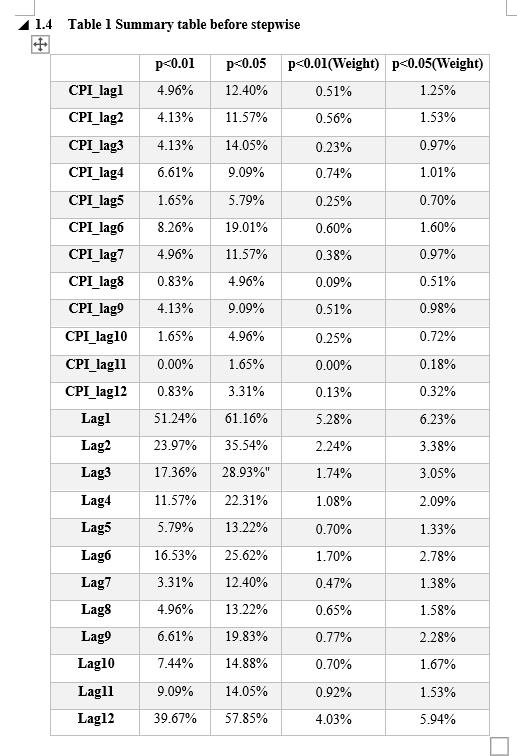
\includegraphics{F:/R workspace/Modelling-UK-inflation-quarterly-/table1.jpg} \\
\midrule
\endhead
论文第一表 \\
\bottomrule
\end{longtable}

\begin{Shaded}
\begin{Highlighting}[]
\NormalTok{a}\OtherTok{=}\FunctionTok{list}\NormalTok{()}
\ControlFlowTok{for}\NormalTok{ (i }\ControlFlowTok{in} \DecValTok{1}\SpecialCharTok{:}\DecValTok{12}\NormalTok{) \{}
\NormalTok{  a[[i]] }\OtherTok{\textless{}{-}} \FunctionTok{lapply}\NormalTok{(regression[}\DecValTok{2}\SpecialCharTok{:}\DecValTok{122}\NormalTok{], }\ControlFlowTok{function}\NormalTok{(x) }\FunctionTok{summary}\NormalTok{(x)}\SpecialCharTok{$}\NormalTok{coefficients[}\FunctionTok{paste0}\NormalTok{(}\StringTok{"CPI\_lag"}\NormalTok{,i), }\DecValTok{4}\NormalTok{])}
  \FunctionTok{print}\NormalTok{(}\FunctionTok{percent}\NormalTok{(}\FunctionTok{length}\NormalTok{(}\FunctionTok{which}\NormalTok{(a[[i]] }\SpecialCharTok{\textless{}} \FloatTok{0.05}\NormalTok{))}\SpecialCharTok{/}\DecValTok{121}\NormalTok{))}
  \CommentTok{\#print(a[[i]])}
\NormalTok{\}}
\end{Highlighting}
\end{Shaded}

\begin{verbatim}
## [1] "12.40%"
## [1] "11.57%"
## [1] "14.05%"
## [1] "9.09%"
## [1] "5.79%"
## [1] "19.01%"
## [1] "11.57%"
## [1] "4.96%"
## [1] "9.09%"
## [1] "4.96%"
## [1] "1.65%"
## [1] "3.31%"
\end{verbatim}

\begin{Shaded}
\begin{Highlighting}[]
\ControlFlowTok{for}\NormalTok{ (i }\ControlFlowTok{in} \DecValTok{1}\SpecialCharTok{:}\DecValTok{12}\NormalTok{) \{}
\NormalTok{  a[[i]] }\OtherTok{\textless{}{-}} \FunctionTok{lapply}\NormalTok{(regression[}\DecValTok{2}\SpecialCharTok{:}\DecValTok{122}\NormalTok{], }\ControlFlowTok{function}\NormalTok{(x) }\FunctionTok{summary}\NormalTok{(x)}\SpecialCharTok{$}\NormalTok{coefficients[}\FunctionTok{paste0}\NormalTok{(}\StringTok{"CPI\_lag"}\NormalTok{,i), }\DecValTok{4}\NormalTok{])}
  
  \FunctionTok{print}\NormalTok{(}\FunctionTok{percent}\NormalTok{(}\FunctionTok{length}\NormalTok{(}\FunctionTok{which}\NormalTok{(a[[i]] }\SpecialCharTok{\textless{}} \FloatTok{0.01}\NormalTok{))}\SpecialCharTok{/}\DecValTok{121}\NormalTok{))}
\NormalTok{\}}
\end{Highlighting}
\end{Shaded}

\begin{verbatim}
## [1] "4.96%"
## [1] "4.13%"
## [1] "4.13%"
## [1] "6.61%"
## [1] "1.65%"
## [1] "8.26%"
## [1] "4.96%"
## [1] "0.83%"
## [1] "4.13%"
## [1] "1.65%"
## [1] "0.00%"
## [1] "0.83%"
\end{verbatim}

\begin{Shaded}
\begin{Highlighting}[]
\ControlFlowTok{for}\NormalTok{ (i }\ControlFlowTok{in} \DecValTok{1}\SpecialCharTok{:}\DecValTok{12}\NormalTok{) \{}
\NormalTok{  a[[i]] }\OtherTok{\textless{}{-}} \FunctionTok{lapply}\NormalTok{(regression[}\DecValTok{2}\SpecialCharTok{:}\DecValTok{122}\NormalTok{], }\ControlFlowTok{function}\NormalTok{(x) }\FunctionTok{summary}\NormalTok{(x)}\SpecialCharTok{$}\NormalTok{coefficients[}\FunctionTok{paste0}\NormalTok{(}\StringTok{"lag"}\NormalTok{,i), }\DecValTok{4}\NormalTok{])}
  \FunctionTok{print}\NormalTok{(}\FunctionTok{percent}\NormalTok{(}\FunctionTok{length}\NormalTok{(}\FunctionTok{which}\NormalTok{(a[[i]] }\SpecialCharTok{\textless{}} \FloatTok{0.05}\NormalTok{))}\SpecialCharTok{/}\DecValTok{121}\NormalTok{))}
  \CommentTok{\#print(a[[i]])}
\NormalTok{\}}
\end{Highlighting}
\end{Shaded}

\begin{verbatim}
## [1] "61.16%"
## [1] "35.54%"
## [1] "28.93%"
## [1] "22.31%"
## [1] "13.22%"
## [1] "25.62%"
## [1] "12.40%"
## [1] "13.22%"
## [1] "19.83%"
## [1] "14.88%"
## [1] "14.05%"
## [1] "57.85%"
\end{verbatim}

\begin{Shaded}
\begin{Highlighting}[]
\ControlFlowTok{for}\NormalTok{ (i }\ControlFlowTok{in} \DecValTok{1}\SpecialCharTok{:}\DecValTok{12}\NormalTok{) \{}
\NormalTok{  a[[i]] }\OtherTok{\textless{}{-}} \FunctionTok{lapply}\NormalTok{(regression[}\DecValTok{2}\SpecialCharTok{:}\DecValTok{122}\NormalTok{], }\ControlFlowTok{function}\NormalTok{(x) }\FunctionTok{summary}\NormalTok{(x)}\SpecialCharTok{$}\NormalTok{coefficients[}\FunctionTok{paste0}\NormalTok{(}\StringTok{"lag"}\NormalTok{,i), }\DecValTok{4}\NormalTok{])}
  
  \FunctionTok{print}\NormalTok{(}\FunctionTok{percent}\NormalTok{(}\FunctionTok{length}\NormalTok{(}\FunctionTok{which}\NormalTok{(a[[i]] }\SpecialCharTok{\textless{}} \FloatTok{0.01}\NormalTok{))}\SpecialCharTok{/}\DecValTok{121}\NormalTok{))}
\NormalTok{\}}
\end{Highlighting}
\end{Shaded}

\begin{verbatim}
## [1] "51.24%"
## [1] "23.97%"
## [1] "17.36%"
## [1] "11.57%"
## [1] "5.79%"
## [1] "16.53%"
## [1] "3.31%"
## [1] "4.96%"
## [1] "6.61%"
## [1] "7.44%"
## [1] "9.09%"
## [1] "39.67%"
\end{verbatim}

\hypertarget{ux540eux4e24ux5217weight}{%
\subsection{后两列(Weight)}\label{ux540eux4e24ux5217weight}}

例如,01部门属于2-15.

\begin{Shaded}
\begin{Highlighting}[]
\CommentTok{\# Weight {-}{-}{-}{-}{-}{-}{-}{-}{-}{-}{-}{-}{-}{-}{-}{-}{-}{-}{-}{-}{-}{-}{-}{-}{-}{-}{-}{-}{-}{-}{-}{-}{-}{-}{-}{-}{-}{-}{-}{-}{-}{-}{-}{-}{-}{-}{-}{-}{-}{-}{-}{-}{-}{-}{-}{-}{-}{-}{-}{-}{-}{-}{-}{-}{-}{-}}
\NormalTok{weight}\OtherTok{\textless{}{-}} \FunctionTok{list}\NormalTok{(}\FloatTok{0.109}\NormalTok{,    }\FloatTok{0.042}\NormalTok{,  }\FloatTok{0.063}\NormalTok{,  }\FloatTok{0.115}\NormalTok{,  }\FloatTok{0.067}\NormalTok{,  }\FloatTok{0.022}\NormalTok{,  }\FloatTok{0.152}\NormalTok{,  }\FloatTok{0.023}\NormalTok{,  }\FloatTok{0.152}\NormalTok{,  }\FloatTok{0.019}\NormalTok{,  }\FloatTok{0.137}\NormalTok{,  }\FloatTok{0.099}
              
\NormalTok{)}
\FunctionTok{Reduce}\NormalTok{(}\StringTok{"+"}\NormalTok{,weight)}
\end{Highlighting}
\end{Shaded}

\begin{verbatim}
## [1] 1
\end{verbatim}

用lapply 把regression 这个list
化成长数据框类型.(多行,5列:term,estimate,std,statitc, pvalue)

\begin{Shaded}
\begin{Highlighting}[]
\NormalTok{tidy\_mods }\OtherTok{\textless{}{-}} \FunctionTok{lapply}\NormalTok{(regression, tidy)}

\ControlFlowTok{for}\NormalTok{ (i }\ControlFlowTok{in} \DecValTok{1}\SpecialCharTok{:}\FunctionTok{length}\NormalTok{(tidy\_mods)) tidy\_mods[[i]]}\SpecialCharTok{$}\NormalTok{mod }\OtherTok{\textless{}{-}} \FunctionTok{names}\NormalTok{(tidy\_mods[i])}
\NormalTok{a }\OtherTok{\textless{}{-}} \FunctionTok{do.call}\NormalTok{(rbind.data.frame, tidy\_mods)}
\FunctionTok{str}\NormalTok{(a)}
\end{Highlighting}
\end{Shaded}

\begin{verbatim}
## tibble[,5] [5,002 x 5] (S3: tbl_df/tbl/data.frame)
##  $ term     : chr [1:5002] "Constant" "lag1" "lag2" "lag3" ...
##  $ estimate : num [1:5002] 0.3623 0.1157 -0.0351 0.0517 0.0445 ...
##  $ std.error: num [1:5002] 0.0754 0.0554 0.0552 0.055 0.0555 ...
##  $ statistic: num [1:5002] 4.802 2.089 -0.636 0.94 0.801 ...
##  $ p.value  : num [1:5002] 2.50e-06 3.75e-02 5.25e-01 3.48e-01 4.23e-01 ...
\end{verbatim}

数数a里面有多少个vat1,就有多少个数据.which(a\$term==``Trend''){[}1{]}代表第一个trend在哪个位置.
每个部门的参数开始于constant,结束于Trend.

42:615行之间lag{[}n{]}且p\textless0.05的*weight{[}1{]}的length

\begin{center}\rule{0.5\linewidth}{0.5pt}\end{center}

01 Food and non-alcoholic beverages \textbf{2-15} 02 Alcoholic
beverages, tobacco and narcotics \textbf{16-21} 03 Clothing and footwear
\textbf{22-27} 04 Housing, water, electricity, gas and other fuels
\textbf{28:40 } 05 Furnishings, household equipment and routine
household maintenance \textbf{41:53 } 06 Health \textbf{54:61 } 07
Transport \textbf{62:76 } 08 Communication \textbf{77:79 } 09 Recreation
and culture \textbf{{[}80:101} 10 Education \textbf{102} 11 Restaurants
and hotels \textbf{103:107} 12 Miscellaneous goods and services
\textbf{108:122}

\begin{center}\rule{0.5\linewidth}{0.5pt}\end{center}

\begin{Shaded}
\begin{Highlighting}[]
\NormalTok{dend}\OtherTok{\textless{}{-}}\FunctionTok{c}\NormalTok{(}\DecValTok{2}\NormalTok{,}\DecValTok{16}\NormalTok{,}\DecValTok{22}\NormalTok{,}\DecValTok{28}\NormalTok{,}\DecValTok{41}\NormalTok{,}\DecValTok{54}\NormalTok{,}\DecValTok{62}\NormalTok{,}\DecValTok{77}\NormalTok{,}\DecValTok{80}\NormalTok{,}\DecValTok{102}\NormalTok{,}\DecValTok{103}\NormalTok{,}\DecValTok{108}\NormalTok{,}\DecValTok{122}\NormalTok{)}\CommentTok{\#这只是每个部门开始的位置}
\ControlFlowTok{for}\NormalTok{ (i }\ControlFlowTok{in} \DecValTok{1}\SpecialCharTok{:}\DecValTok{12}\NormalTok{) \{}
  \FunctionTok{assign}\NormalTok{(}\FunctionTok{paste0}\NormalTok{(}\StringTok{"a"}\NormalTok{,i),}
\NormalTok{         a[(}\FunctionTok{which}\NormalTok{(a}\SpecialCharTok{$}\NormalTok{term}\SpecialCharTok{==}\StringTok{"Constant"}\NormalTok{)[dend[i]])}\SpecialCharTok{:}\NormalTok{(}\FunctionTok{which}\NormalTok{(a}\SpecialCharTok{$}\NormalTok{term}\SpecialCharTok{==}\StringTok{"Trend"}\NormalTok{)[dend[i}\SpecialCharTok{+}\DecValTok{1}\NormalTok{]}\SpecialCharTok{{-}}\DecValTok{1}\NormalTok{]),])}
\NormalTok{\}}
\end{Highlighting}
\end{Shaded}

第一个constant的位置,到下一个Trend-1的位置. 第一个部门是2:15,
开始的标志是第二个constant的位置(dend{[}1{]}),结束于第15个Trend的位置(dend{[}2{]}-1的trend).
\textbf{之所以不是直接开始于constant{[}dend{[}1{]}{]},结束于trend{[}dend{[}1{]}{]},是因为dend只是开始位置的集合(constant)而并不是结束的位置(trend).}

\emph{如果constant{[}dend{[}1{]}{]}---trend{[}dend{[}1{]}{]},这代表第二个(dend{[}1{]}=2)
constant的开始到第二个trend的结束.只是一个class.}

\textbf{如果constant{[}dend{[}1{]}{]}---trend{[}dend{[}2{]}{]},这代表第二个constant的开始到第16(dend{[}2{]}=16)
个trend的结束.我需要的是到第15个结束}

a1中lag1小于0.01的.a2中lag2小于0.01的.

\textbf{我想要的是a1中的lag1-12且小于0.01的个数×weight{[}1{]}.}

这样就是{[}1{]}\textless-a1的lag1且小于0.01的\emph{weight{[}1{]},{[}2{]}\textless-a2
lag1且小于0.01的个数}weight{[}2{]}

尝试先后循环 总共应该有多少个结果啊? a1{[}lag1:12{]} 12*12=144个

首先生成一个12*12的dataframe, 行是lag1-12, 列是a1:a12 十二个部门.
双循环,每个部门循环把lag1-lag12
循环一边存储在a\_lag\_0.01{[},i{]}列里,然后再循环剩下11个部门.

\hypertarget{a_lag.0.01}{%
\subsubsection{a\_lag.0.01}\label{a_lag.0.01}}

\begin{Shaded}
\begin{Highlighting}[]
\NormalTok{a\_lag.}\FloatTok{0.01}\OtherTok{\textless{}{-}}\FunctionTok{data.frame}\NormalTok{( }\AttributeTok{row.names =}  \FunctionTok{paste0}\NormalTok{(}\StringTok{"lag"}\NormalTok{,}\DecValTok{1}\SpecialCharTok{:}\DecValTok{12}\NormalTok{),}
                   \FunctionTok{matrix}\NormalTok{(}\AttributeTok{nrow=}\DecValTok{12}\NormalTok{, }\AttributeTok{ncol=}\DecValTok{12}\NormalTok{, ) ) }

\FunctionTok{colnames}\NormalTok{(a\_lag.}\FloatTok{0.01}\NormalTok{)}\OtherTok{\textless{}{-}}\FunctionTok{c}\NormalTok{(}\FunctionTok{paste0}\NormalTok{(}\StringTok{"a"}\NormalTok{,}\DecValTok{1}\SpecialCharTok{:}\DecValTok{12}\NormalTok{))}
\NormalTok{i}\OtherTok{\textless{}{-}}\DecValTok{1}\CommentTok{\#i=a,j=lag}
\ControlFlowTok{while}\NormalTok{ (i }\SpecialCharTok{\textless{}=}\DecValTok{12}\NormalTok{) \{}
  \ControlFlowTok{for}\NormalTok{ (j }\ControlFlowTok{in} \DecValTok{1}\SpecialCharTok{:}\DecValTok{12}\NormalTok{) \{}
\NormalTok{ a\_lag.}\FloatTok{0.01}\NormalTok{ [j,i]  }\OtherTok{\textless{}{-}}
  \FunctionTok{length}\NormalTok{( }\FunctionTok{which}\NormalTok{((}\FunctionTok{get}\NormalTok{(}\FunctionTok{paste0}\NormalTok{(}\StringTok{"a"}\NormalTok{,i)))}\SpecialCharTok{$}\NormalTok{term}\SpecialCharTok{==}\FunctionTok{paste0}\NormalTok{(}\StringTok{"lag"}\NormalTok{,j)}\SpecialCharTok{\&}\NormalTok{(}\FunctionTok{get}\NormalTok{(}\FunctionTok{paste0}\NormalTok{(}\StringTok{"a"}\NormalTok{,i)))}\SpecialCharTok{$}\NormalTok{p.value}\SpecialCharTok{\textless{}}\FloatTok{0.01}\NormalTok{)}
\NormalTok{  )}\SpecialCharTok{*}\NormalTok{weight[[i]]}
\NormalTok{  \}}
\NormalTok{  i}\OtherTok{\textless{}{-}}\NormalTok{i}\SpecialCharTok{+}\DecValTok{1}
\NormalTok{\}}
\end{Highlighting}
\end{Shaded}

a8全都是0. 证实了一下确实. 有在0.05显著的,但是没有在0.01显著的.

\begin{verbatim}
## 
## =============================================================================
##                                        Dependent variable:                   
##                     ---------------------------------------------------------
##                                             COPY[, x]                        
##                     FOOD AND NON-ALCOHOLIC BEVERAGES  FOOD  BREAD and CEREALS
## -----------------------------------------------------------------------------
## Constant                         -0.42               -1.66*       -0.39      
## lag1                             0.002               -0.15*       0.01       
## lag2                              0.08               -0.03        0.07       
## lag3                              0.07               -0.01        0.06       
## lag4                             -0.09               -0.04        -0.07      
## lag5                             -0.06               -0.02        -0.06      
## lag6                             -0.03               -0.04        -0.04      
## lag7                              0.01               -0.04        0.04       
## lag8                             -0.03               -0.05        -0.04      
## lag9                             0.12*               0.003        0.13*      
## lag10                             0.09               0.002        0.08       
## lag11                            -0.06                0.06        -0.05      
## lag12                            -0.03                0.08        -0.06      
## CPI_lag1                         -0.16               -0.46        -0.15      
## CPI_lag2                         -0.06                0.63        -0.12      
## CPI_lag3                         0.49*                0.46        0.52*      
## CPI_lag4                         -0.23                0.35        -0.25      
## CPI_lag5                          0.38                0.30        0.41       
## CPI_lag6                         -0.16                0.58        -0.20      
## CPI_lag7                         -0.06               -0.88        -0.07      
## CPI_lag8                          0.26                0.75        0.25       
## CPI_lag9                         -0.13                0.70        -0.21      
## CPI_lag10                        -0.02                0.89        -0.05      
## CPI_lag11                         0.19               -0.27        0.27       
## CPI_lag12                         0.04               -0.50        0.09       
## time_Aug                         -0.04                0.22        -0.11      
## time_Dec                          0.25                0.78        0.26       
## time_Feb                          0.61               4.27**       0.40       
## time_Jan                         -0.21                0.53        -0.24      
## time_Jul                         -0.42                1.18        -0.51      
## time_Jun                          0.35                0.61        0.39       
## time_Mar                         -0.06               2.04*        -0.23      
## time_May                         -0.27               2.74**       -0.39      
## time_Nov                         -0.22                1.75        -0.31      
## time_Oct                          0.12                1.39        0.05       
## time_Sep                          0.24               2.28*        0.13       
## VAT1                            -2.24**              -1.05       -2.35**     
## VAT2                              0.88                0.10        0.98       
## VAT3                              0.81               -0.02        0.94       
## Recession                         0.15                0.35        0.14       
## Trend                           0.002**              0.001       0.002**     
## -----------------------------------------------------------------------------
## Observations                      324                 324          324       
## R2                                0.23                0.27        0.22       
## Adjusted R2                       0.12                0.17        0.11       
## Residual Std. Error               0.65                1.63        0.70       
## F Statistic                      2.14**              2.63**      2.04**      
## =============================================================================
## Note:                                         *p<0.05; **p<0.01; ***p<[0.***]
\end{verbatim}

\hypertarget{a_lag.0.05}{%
\subsubsection{a\_lag.0.05}\label{a_lag.0.05}}

\begin{Shaded}
\begin{Highlighting}[]
\NormalTok{a\_lag.}\FloatTok{0.05}\OtherTok{\textless{}{-}}\FunctionTok{data.frame}\NormalTok{( }\AttributeTok{row.names =}  \FunctionTok{paste0}\NormalTok{(}\StringTok{"lag"}\NormalTok{,}\DecValTok{1}\SpecialCharTok{:}\DecValTok{12}\NormalTok{),}
                   \FunctionTok{matrix}\NormalTok{(}\AttributeTok{nrow=}\DecValTok{12}\NormalTok{, }\AttributeTok{ncol=}\DecValTok{12}\NormalTok{, ) ) }

\FunctionTok{colnames}\NormalTok{(a\_lag.}\FloatTok{0.05}\NormalTok{)}\OtherTok{\textless{}{-}}\FunctionTok{c}\NormalTok{(}\FunctionTok{paste0}\NormalTok{(}\StringTok{"a"}\NormalTok{,}\DecValTok{1}\SpecialCharTok{:}\DecValTok{12}\NormalTok{))}
\NormalTok{i}\OtherTok{\textless{}{-}}\DecValTok{1}\CommentTok{\#i=a,j=lag}
\ControlFlowTok{while}\NormalTok{ (i }\SpecialCharTok{\textless{}=}\DecValTok{12}\NormalTok{) \{}
  \ControlFlowTok{for}\NormalTok{ (j }\ControlFlowTok{in} \DecValTok{1}\SpecialCharTok{:}\DecValTok{12}\NormalTok{) \{}
\NormalTok{ a\_lag.}\FloatTok{0.05}\NormalTok{ [j,i]  }\OtherTok{\textless{}{-}}
  \FunctionTok{length}\NormalTok{( }\FunctionTok{which}\NormalTok{((}\FunctionTok{get}\NormalTok{(}\FunctionTok{paste0}\NormalTok{(}\StringTok{"a"}\NormalTok{,i)))}\SpecialCharTok{$}\NormalTok{term}\SpecialCharTok{==}\FunctionTok{paste0}\NormalTok{(}\StringTok{"lag"}\NormalTok{,j)}\SpecialCharTok{\&}\NormalTok{(}\FunctionTok{get}\NormalTok{(}\FunctionTok{paste0}\NormalTok{(}\StringTok{"a"}\NormalTok{,i)))}\SpecialCharTok{$}\NormalTok{p.value}\SpecialCharTok{\textless{}}\FloatTok{0.05}\NormalTok{)}
\NormalTok{  )}\SpecialCharTok{*}\NormalTok{weight[[i]]}
\NormalTok{  \}}
\NormalTok{  i}\OtherTok{\textless{}{-}}\NormalTok{i}\SpecialCharTok{+}\DecValTok{1}
\NormalTok{\}}
\end{Highlighting}
\end{Shaded}

\hypertarget{a_cpi.0.01}{%
\subsubsection{a\_cpi.0.01}\label{a_cpi.0.01}}

\begin{Shaded}
\begin{Highlighting}[]
\NormalTok{a\_cpi.}\FloatTok{0.01}\OtherTok{\textless{}{-}}\FunctionTok{data.frame}\NormalTok{( }\AttributeTok{row.names =}  \FunctionTok{paste0}\NormalTok{(}\StringTok{"CPI\_lag"}\NormalTok{,}\DecValTok{1}\SpecialCharTok{:}\DecValTok{12}\NormalTok{),}
                   \FunctionTok{matrix}\NormalTok{(}\AttributeTok{nrow=}\DecValTok{12}\NormalTok{, }\AttributeTok{ncol=}\DecValTok{12}\NormalTok{, ) ) }

\FunctionTok{colnames}\NormalTok{(a\_cpi.}\FloatTok{0.01}\NormalTok{)}\OtherTok{\textless{}{-}}\FunctionTok{c}\NormalTok{(}\FunctionTok{paste0}\NormalTok{(}\StringTok{"a"}\NormalTok{,}\DecValTok{1}\SpecialCharTok{:}\DecValTok{12}\NormalTok{))}
\NormalTok{i}\OtherTok{\textless{}{-}}\DecValTok{1}\CommentTok{\#i=a,j=lag}
\ControlFlowTok{while}\NormalTok{ (i }\SpecialCharTok{\textless{}=}\DecValTok{12}\NormalTok{) \{}
  \ControlFlowTok{for}\NormalTok{ (j }\ControlFlowTok{in} \DecValTok{1}\SpecialCharTok{:}\DecValTok{12}\NormalTok{) \{}
\NormalTok{ a\_cpi.}\FloatTok{0.01}\NormalTok{ [j,i]  }\OtherTok{\textless{}{-}}
  \FunctionTok{length}\NormalTok{( }\FunctionTok{which}\NormalTok{((}\FunctionTok{get}\NormalTok{(}\FunctionTok{paste0}\NormalTok{(}\StringTok{"a"}\NormalTok{,i)))}\SpecialCharTok{$}\NormalTok{term}\SpecialCharTok{==}\FunctionTok{paste0}\NormalTok{(}\StringTok{"CPI\_lag"}\NormalTok{,j)}\SpecialCharTok{\&}\NormalTok{(}\FunctionTok{get}\NormalTok{(}\FunctionTok{paste0}\NormalTok{(}\StringTok{"a"}\NormalTok{,i)))}\SpecialCharTok{$}\NormalTok{p.value}\SpecialCharTok{\textless{}}\FloatTok{0.01}\NormalTok{)}
\NormalTok{  )}\SpecialCharTok{*}\NormalTok{weight[[i]]}
\NormalTok{  \}}
\NormalTok{  i}\OtherTok{\textless{}{-}}\NormalTok{i}\SpecialCharTok{+}\DecValTok{1}
\NormalTok{\}}
\end{Highlighting}
\end{Shaded}

\hypertarget{a_cpi.0.05}{%
\subsubsection{a\_cpi.0.05}\label{a_cpi.0.05}}

\begin{Shaded}
\begin{Highlighting}[]
\NormalTok{a\_cpi.}\FloatTok{0.05}\OtherTok{\textless{}{-}}\FunctionTok{data.frame}\NormalTok{( }\AttributeTok{row.names =}  \FunctionTok{paste0}\NormalTok{(}\StringTok{"CPI\_lag"}\NormalTok{,}\DecValTok{1}\SpecialCharTok{:}\DecValTok{12}\NormalTok{),}
                   \FunctionTok{matrix}\NormalTok{(}\AttributeTok{nrow=}\DecValTok{12}\NormalTok{, }\AttributeTok{ncol=}\DecValTok{12}\NormalTok{, ) ) }

\FunctionTok{colnames}\NormalTok{(a\_cpi.}\FloatTok{0.05}\NormalTok{)}\OtherTok{\textless{}{-}}\FunctionTok{c}\NormalTok{(}\FunctionTok{paste0}\NormalTok{(}\StringTok{"a"}\NormalTok{,}\DecValTok{1}\SpecialCharTok{:}\DecValTok{12}\NormalTok{))}
\NormalTok{i}\OtherTok{\textless{}{-}}\DecValTok{1}\CommentTok{\#i=a,j=lag}
\ControlFlowTok{while}\NormalTok{ (i }\SpecialCharTok{\textless{}=}\DecValTok{12}\NormalTok{) \{}
  \ControlFlowTok{for}\NormalTok{ (j }\ControlFlowTok{in} \DecValTok{1}\SpecialCharTok{:}\DecValTok{12}\NormalTok{) \{}
\NormalTok{ a\_cpi.}\FloatTok{0.05}\NormalTok{ [j,i]  }\OtherTok{\textless{}{-}}
  \FunctionTok{length}\NormalTok{( }\FunctionTok{which}\NormalTok{((}\FunctionTok{get}\NormalTok{(}\FunctionTok{paste0}\NormalTok{(}\StringTok{"a"}\NormalTok{,i)))}\SpecialCharTok{$}\NormalTok{term}\SpecialCharTok{==}\FunctionTok{paste0}\NormalTok{(}\StringTok{"CPI\_lag"}\NormalTok{,j)}\SpecialCharTok{\&}\NormalTok{(}\FunctionTok{get}\NormalTok{(}\FunctionTok{paste0}\NormalTok{(}\StringTok{"a"}\NormalTok{,i)))}\SpecialCharTok{$}\NormalTok{p.value}\SpecialCharTok{\textless{}}\FloatTok{0.05}\NormalTok{)}
\NormalTok{  )}\SpecialCharTok{*}\NormalTok{weight[[i]]}
\NormalTok{  \}}
\NormalTok{  i}\OtherTok{\textless{}{-}}\NormalTok{i}\SpecialCharTok{+}\DecValTok{1}
\NormalTok{\}}
\end{Highlighting}
\end{Shaded}

\[
\frac{\text{部门}1\text{显著个数}*weight\left[ 1 \right] +.....+}{121}
\] 把a\_cpi.0.05这四个表, 每行加起来/121 就是结果.
一行一个结果,每个表有12行,共4个表,\textbf{4×12=48}个结果.
首先生成存放结果的 24行×2列的dataframe

\hypertarget{ux6240ux6709table1ux7684ux7ed3ux679cux90fdux5199ux5165ux8fd9ux6b21ux8981ux751fux6210244ux7684dataframe}{%
\section{所有table1的结果都写入,这次要生成24*4的dataframe}\label{ux6240ux6709table1ux7684ux7ed3ux679cux90fdux5199ux5165ux8fd9ux6b21ux8981ux751fux6210244ux7684dataframe}}

\begin{Shaded}
\begin{Highlighting}[]
\NormalTok{table1weight}\OtherTok{\textless{}{-}}\FunctionTok{data.frame}\NormalTok{( }\FunctionTok{matrix}\NormalTok{(}\AttributeTok{nrow=}\DecValTok{24}\NormalTok{, }\AttributeTok{ncol=}\DecValTok{4}\NormalTok{, )   )}
\FunctionTok{colnames}\NormalTok{(table1weight)}\OtherTok{\textless{}{-}}\FunctionTok{c}\NormalTok{(}\StringTok{"p\textless{}0.01"}\NormalTok{,}\StringTok{"p\textless{}0.05"}\NormalTok{,}\StringTok{"p\textless{}0.01(Weight)"}\NormalTok{,}\StringTok{"p\textless{}0.05(Weight)"}\NormalTok{)}
\FunctionTok{rownames}\NormalTok{(table1weight)}\OtherTok{\textless{}{-}}\FunctionTok{c}\NormalTok{(}\FunctionTok{paste0}\NormalTok{(}\StringTok{"CPI\_lag"}\NormalTok{,}\DecValTok{1}\SpecialCharTok{:}\DecValTok{12}\NormalTok{),}\FunctionTok{paste0}\NormalTok{(}\StringTok{"lag"}\NormalTok{,}\DecValTok{1}\SpecialCharTok{:}\DecValTok{12}\NormalTok{))}
\end{Highlighting}
\end{Shaded}

写入结果 一个没有cpi的a dataframe,删除前14行

\begin{Shaded}
\begin{Highlighting}[]
\NormalTok{nocpi}\OtherTok{\textless{}{-}}\NormalTok{a[}\SpecialCharTok{{-}}\FunctionTok{c}\NormalTok{(}\DecValTok{1}\SpecialCharTok{:}\DecValTok{41}\NormalTok{),]}
\end{Highlighting}
\end{Shaded}

\begin{Shaded}
\begin{Highlighting}[]
\ControlFlowTok{for}\NormalTok{ (i }\ControlFlowTok{in} \DecValTok{1}\SpecialCharTok{:}\DecValTok{12}\NormalTok{) \{}\CommentTok{\#前两列}
\NormalTok{  table1weight[i,}\DecValTok{1}\NormalTok{]}\OtherTok{\textless{}{-}}\FunctionTok{percent}\NormalTok{((}\FunctionTok{length}\NormalTok{( }\FunctionTok{which}\NormalTok{(nocpi}\SpecialCharTok{$}\NormalTok{term}\SpecialCharTok{==}\FunctionTok{paste0}\NormalTok{(}\StringTok{"CPI\_lag"}\NormalTok{,i)}\SpecialCharTok{\&}\NormalTok{(nocpi}\SpecialCharTok{$}\NormalTok{p.value}\SpecialCharTok{\textless{}}\FloatTok{0.01}\NormalTok{))))}\SpecialCharTok{/}\DecValTok{121}\NormalTok{)}
\NormalTok{   table1weight[i}\SpecialCharTok{+}\DecValTok{12}\NormalTok{,}\DecValTok{1}\NormalTok{]}\OtherTok{\textless{}{-}}\FunctionTok{percent}\NormalTok{((}\FunctionTok{length}\NormalTok{( }\FunctionTok{which}\NormalTok{(nocpi}\SpecialCharTok{$}\NormalTok{term}\SpecialCharTok{==}\FunctionTok{paste0}\NormalTok{(}\StringTok{"lag"}\NormalTok{,i)}\SpecialCharTok{\&}\NormalTok{(nocpi}\SpecialCharTok{$}\NormalTok{p.value}\SpecialCharTok{\textless{}}\FloatTok{0.01}\NormalTok{))))}\SpecialCharTok{/}\DecValTok{121}\NormalTok{)}
\NormalTok{   table1weight[i,}\DecValTok{2}\NormalTok{]}\OtherTok{\textless{}{-}}\FunctionTok{percent}\NormalTok{((}\FunctionTok{length}\NormalTok{( }\FunctionTok{which}\NormalTok{(nocpi}\SpecialCharTok{$}\NormalTok{term}\SpecialCharTok{==}\FunctionTok{paste0}\NormalTok{(}\StringTok{"CPI\_lag"}\NormalTok{,i)}\SpecialCharTok{\&}\NormalTok{(nocpi}\SpecialCharTok{$}\NormalTok{p.value}\SpecialCharTok{\textless{}}\FloatTok{0.05}\NormalTok{))))}\SpecialCharTok{/}\DecValTok{121}\NormalTok{)}
\NormalTok{      table1weight[i}\SpecialCharTok{+}\DecValTok{12}\NormalTok{,}\DecValTok{2}\NormalTok{]}\OtherTok{\textless{}{-}}\FunctionTok{percent}\NormalTok{((}\FunctionTok{length}\NormalTok{( }\FunctionTok{which}\NormalTok{(nocpi}\SpecialCharTok{$}\NormalTok{term}\SpecialCharTok{==}\FunctionTok{paste0}\NormalTok{(}\StringTok{"lag"}\NormalTok{,i)}\SpecialCharTok{\&}\NormalTok{(nocpi}\SpecialCharTok{$}\NormalTok{p.value}\SpecialCharTok{\textless{}}\FloatTok{0.05}\NormalTok{))))}\SpecialCharTok{/}\DecValTok{121}\NormalTok{)}
      \CommentTok{\#后两列}
\NormalTok{    table1weight[i,}\DecValTok{3}\NormalTok{]}\OtherTok{\textless{}{-}}\FunctionTok{percent}\NormalTok{(}\FunctionTok{sum}\NormalTok{(a\_cpi.}\FloatTok{0.01}\NormalTok{[}\FunctionTok{paste0}\NormalTok{(}\StringTok{"CPI\_lag"}\NormalTok{,i),])      }\SpecialCharTok{/}\DecValTok{121}\NormalTok{)}
\NormalTok{    table1weight[i}\SpecialCharTok{+}\DecValTok{12}\NormalTok{,}\DecValTok{3}\NormalTok{]}\OtherTok{\textless{}{-}}\FunctionTok{percent}\NormalTok{(}\FunctionTok{sum}\NormalTok{(a\_lag.}\FloatTok{0.01}\NormalTok{[}\FunctionTok{paste0}\NormalTok{(}\StringTok{"lag"}\NormalTok{,i),])}\SpecialCharTok{/}\DecValTok{121}\NormalTok{)}
\NormalTok{    table1weight[i,}\DecValTok{4}\NormalTok{]}\OtherTok{\textless{}{-}}\FunctionTok{percent}\NormalTok{(}\FunctionTok{sum}\NormalTok{(a\_cpi.}\FloatTok{0.05}\NormalTok{[}\FunctionTok{paste0}\NormalTok{(}\StringTok{"CPI\_lag"}\NormalTok{,i),])}\SpecialCharTok{/}\DecValTok{121}\NormalTok{)}
\NormalTok{    table1weight[i}\SpecialCharTok{+}\DecValTok{12}\NormalTok{,}\DecValTok{4}\NormalTok{]}\OtherTok{\textless{}{-}}\FunctionTok{percent}\NormalTok{(}\FunctionTok{sum}\NormalTok{(a\_lag.}\FloatTok{0.05}\NormalTok{[}\FunctionTok{paste0}\NormalTok{(}\StringTok{"lag"}\NormalTok{,i),])}\SpecialCharTok{/}\DecValTok{121}\NormalTok{)}
    
\NormalTok{\}}
\end{Highlighting}
\end{Shaded}

flextable 写入word

\begin{Shaded}
\begin{Highlighting}[]
\NormalTok{ft1}\OtherTok{\textless{}{-}}\FunctionTok{flextable}\NormalTok{(table1weight }\SpecialCharTok{\%\textgreater{}\%} \FunctionTok{rownames\_to\_column}\NormalTok{(}\StringTok{"column name"}\NormalTok{))}




\FunctionTok{save\_as\_docx}\NormalTok{(}\StringTok{"Summary table before stepwise"} \OtherTok{=}\NormalTok{ ft1, }\AttributeTok{path =} \StringTok{"F:/R workspace/Modelling{-}UK{-}inflation{-}quarterly{-}/table1.docx"}\NormalTok{)}
\end{Highlighting}
\end{Shaded}

\begin{center}\rule{0.5\linewidth}{0.5pt}\end{center}

\hypertarget{table-2-stepwise-summary-table}{%
\section{Table 2 Stepwise Summary
Table}\label{table-2-stepwise-summary-table}}

\hypertarget{stepwise-function}{%
\subsection{stepwise function}\label{stepwise-function}}

\begin{Shaded}
\begin{Highlighting}[]
\CommentTok{\# function {-}{-}{-}{-}{-}{-}{-}{-}{-}{-}{-}{-}{-}{-}{-}{-}{-}{-}{-}{-}{-}{-}{-}{-}{-}{-}{-}{-}{-}{-}{-}{-}{-}{-}{-}{-}{-}{-}{-}{-}{-}{-}{-}{-}{-}{-}{-}{-}{-}{-}{-}{-}{-}{-}{-}{-}{-}{-}{-}{-}{-}{-}{-}{-}}


\CommentTok{\# Automated model selection}
\CommentTok{\# Author      : Joris Meys}
\CommentTok{\# version     : 0.2}
\CommentTok{\# date        : 12/01/09}

\CommentTok{\#CHANGE LOG}
\CommentTok{\# 0.2   : check for empty scopevar vector}

\CommentTok{\# \#CHANGE LOG {-}{-}{-}{-}{-}{-}{-}{-}{-}{-}{-}{-}{-}{-}{-}{-}{-}{-}{-}{-}{-}{-}{-}{-}{-}{-}{-}{-}{-}{-}{-}{-}{-}{-}{-}{-}{-}{-}{-}{-}{-}{-}{-}{-}{-}{-}{-}{-}{-}{-}{-}{-}{-}{-}{-}{-}{-}{-}{-}{-}{-}}



\CommentTok{\# Function has.interaction checks whether x is part of a term in terms}
\CommentTok{\# terms is a vector with names of terms from a model}
\NormalTok{has.interaction }\OtherTok{\textless{}{-}} \ControlFlowTok{function}\NormalTok{(x,terms)\{}
\NormalTok{  out }\OtherTok{\textless{}{-}} \FunctionTok{sapply}\NormalTok{(terms,}\ControlFlowTok{function}\NormalTok{(i)\{}
    \FunctionTok{sum}\NormalTok{(}\DecValTok{1}\SpecialCharTok{{-}}\NormalTok{(}\FunctionTok{strsplit}\NormalTok{(x,}\StringTok{":"}\NormalTok{)[[}\DecValTok{1}\NormalTok{]] }\SpecialCharTok{\%in\%} \FunctionTok{strsplit}\NormalTok{(i,}\StringTok{":"}\NormalTok{)[[}\DecValTok{1}\NormalTok{]]))}\SpecialCharTok{==}\DecValTok{0}
\NormalTok{  \})}
  \FunctionTok{return}\NormalTok{(}\FunctionTok{sum}\NormalTok{(out)}\SpecialCharTok{\textgreater{}}\DecValTok{0}\NormalTok{)}
\NormalTok{\}}

\CommentTok{\# Function Model.select}
\CommentTok{\# model is the lm object of the full model}
\CommentTok{\# keep is a list of model terms to keep in the model at all times}
\CommentTok{\# sig gives the significance for removal of a variable. Can be 0.1 too (see SPSS)}
\CommentTok{\# verbose=T gives the F{-}tests, dropped var and resulting model after }
\NormalTok{model.select }\OtherTok{\textless{}{-}} \ControlFlowTok{function}\NormalTok{(model,keep,}\AttributeTok{sig=}\FloatTok{0.05}\NormalTok{,}\AttributeTok{verbose=}\NormalTok{F)\{}
\NormalTok{  counter}\OtherTok{=}\DecValTok{1}
  \CommentTok{\# check input}
  \ControlFlowTok{if}\NormalTok{(}\SpecialCharTok{!}\FunctionTok{is}\NormalTok{(model,}\StringTok{"lm"}\NormalTok{)) }\FunctionTok{stop}\NormalTok{(}\FunctionTok{paste}\NormalTok{(}\FunctionTok{deparse}\NormalTok{(}\FunctionTok{substitute}\NormalTok{(model)),}\StringTok{"is not an lm object}\SpecialCharTok{\textbackslash{}n}\StringTok{"}\NormalTok{))}
  \CommentTok{\# calculate scope for drop1 function}
\NormalTok{  terms }\OtherTok{\textless{}{-}} \FunctionTok{attr}\NormalTok{(model}\SpecialCharTok{$}\NormalTok{terms,}\StringTok{"term.labels"}\NormalTok{)}
  \ControlFlowTok{if}\NormalTok{(}\FunctionTok{missing}\NormalTok{(keep))\{ }\CommentTok{\# set scopevars to all terms}
\NormalTok{    scopevars }\OtherTok{\textless{}{-}}\NormalTok{ terms}
\NormalTok{  \} }\ControlFlowTok{else}\NormalTok{\{            }\CommentTok{\# select the scopevars if keep is used}
\NormalTok{    index }\OtherTok{\textless{}{-}} \FunctionTok{match}\NormalTok{(keep,terms)}
    \CommentTok{\# check if all is specified correctly}
    \ControlFlowTok{if}\NormalTok{(}\FunctionTok{sum}\NormalTok{(}\FunctionTok{is.na}\NormalTok{(index))}\SpecialCharTok{\textgreater{}}\DecValTok{0}\NormalTok{)\{}
\NormalTok{      novar }\OtherTok{\textless{}{-}}\NormalTok{ keep[}\FunctionTok{is.na}\NormalTok{(index)]}
      \FunctionTok{warning}\NormalTok{(}\FunctionTok{paste}\NormalTok{(}
        \FunctionTok{c}\NormalTok{(novar,}\StringTok{"cannot be found in the model"}\NormalTok{,}
          \StringTok{"}\SpecialCharTok{\textbackslash{}n}\StringTok{These terms are ignored in the model selection."}\NormalTok{),}
        \AttributeTok{collapse=}\StringTok{" "}\NormalTok{))}
\NormalTok{      index }\OtherTok{\textless{}{-}} \FunctionTok{as.vector}\NormalTok{(}\FunctionTok{na.omit}\NormalTok{(index))}
\NormalTok{    \}}
\NormalTok{    scopevars }\OtherTok{\textless{}{-}}\NormalTok{ terms[}\SpecialCharTok{{-}}\NormalTok{index]}
\NormalTok{  \}}
  
  \CommentTok{\# Backward model selection : }
  
  \ControlFlowTok{while}\NormalTok{(T)\{}
    \CommentTok{\# extract the test statistics from drop.}
\NormalTok{    test }\OtherTok{\textless{}{-}} \FunctionTok{drop1}\NormalTok{(model, }\AttributeTok{scope=}\NormalTok{scopevars,}\AttributeTok{test=}\StringTok{"F"}\NormalTok{)}
    
    \ControlFlowTok{if}\NormalTok{(verbose)\{}
      \FunctionTok{cat}\NormalTok{(}\StringTok{"{-}{-}{-}{-}{-}{-}{-}{-}{-}{-}{-}{-}{-}STEP "}\NormalTok{,counter,}\StringTok{"{-}{-}{-}{-}{-}{-}{-}{-}{-}{-}{-}{-}{-}}\SpecialCharTok{\textbackslash{}n}\StringTok{"}\NormalTok{,}
          \StringTok{"The drop statistics : }\SpecialCharTok{\textbackslash{}n}\StringTok{"}\NormalTok{)}
      \FunctionTok{print}\NormalTok{(test)}
\NormalTok{    \}}
    
\NormalTok{    pval }\OtherTok{\textless{}{-}}\NormalTok{ test[,}\FunctionTok{dim}\NormalTok{(test)[}\DecValTok{2}\NormalTok{]]}
    
    \FunctionTok{names}\NormalTok{(pval) }\OtherTok{\textless{}{-}} \FunctionTok{rownames}\NormalTok{(test)}
\NormalTok{    pval }\OtherTok{\textless{}{-}} \FunctionTok{sort}\NormalTok{(pval,}\AttributeTok{decreasing=}\NormalTok{T)}
    
    \ControlFlowTok{if}\NormalTok{(}\FunctionTok{sum}\NormalTok{(}\FunctionTok{is.na}\NormalTok{(pval))}\SpecialCharTok{\textgreater{}}\DecValTok{0}\NormalTok{) }\FunctionTok{stop}\NormalTok{(}\FunctionTok{paste}\NormalTok{(}\StringTok{"Model"}\NormalTok{,}
                                      \FunctionTok{deparse}\NormalTok{(}\FunctionTok{substitute}\NormalTok{(model)),}\StringTok{"is invalid. Check if all coefficients are estimated."}\NormalTok{))}
    
    \CommentTok{\# check if all significant}
    \ControlFlowTok{if}\NormalTok{(pval[}\DecValTok{1}\NormalTok{]}\SpecialCharTok{\textless{}}\NormalTok{sig) }\ControlFlowTok{break} \CommentTok{\# stops the loop if all remaining vars are sign.}
    
    \CommentTok{\# select var to drop}
\NormalTok{    i}\OtherTok{=}\DecValTok{1}
    \ControlFlowTok{while}\NormalTok{(T)\{}
\NormalTok{      dropvar }\OtherTok{\textless{}{-}} \FunctionTok{names}\NormalTok{(pval)[i]}
\NormalTok{      check.terms }\OtherTok{\textless{}{-}}\NormalTok{ terms[}\SpecialCharTok{{-}}\FunctionTok{match}\NormalTok{(dropvar,terms)]}
\NormalTok{      x }\OtherTok{\textless{}{-}} \FunctionTok{has.interaction}\NormalTok{(dropvar,check.terms)}
      \ControlFlowTok{if}\NormalTok{(x)\{i}\OtherTok{=}\NormalTok{i}\SpecialCharTok{+}\DecValTok{1}\NormalTok{;}\ControlFlowTok{next}\NormalTok{\} }\ControlFlowTok{else}\NormalTok{ \{}\ControlFlowTok{break}\NormalTok{\}              }
\NormalTok{    \} }\CommentTok{\# end while(T) drop var}
    
    \ControlFlowTok{if}\NormalTok{(pval[i]}\SpecialCharTok{\textless{}}\NormalTok{sig) }\ControlFlowTok{break} \CommentTok{\# stops the loop if var to remove is significant}
    
    \ControlFlowTok{if}\NormalTok{(verbose)\{}
      \FunctionTok{cat}\NormalTok{(}\StringTok{"}\SpecialCharTok{\textbackslash{}n}\StringTok{{-}{-}{-}{-}{-}{-}{-}{-}}\SpecialCharTok{\textbackslash{}n}\StringTok{Term dropped in step"}\NormalTok{,counter,}\StringTok{":"}\NormalTok{,dropvar,}\StringTok{"}\SpecialCharTok{\textbackslash{}n}\StringTok{{-}{-}{-}{-}{-}{-}{-}{-}}\SpecialCharTok{\textbackslash{}n\textbackslash{}n}\StringTok{"}\NormalTok{)              }
\NormalTok{    \}}
    
    \CommentTok{\#update terms, scopevars and model}
\NormalTok{    scopevars }\OtherTok{\textless{}{-}}\NormalTok{ scopevars[}\SpecialCharTok{{-}}\FunctionTok{match}\NormalTok{(dropvar,scopevars)]}
\NormalTok{    terms }\OtherTok{\textless{}{-}}\NormalTok{ terms[}\SpecialCharTok{{-}}\FunctionTok{match}\NormalTok{(dropvar,terms)]}
    
\NormalTok{    formul }\OtherTok{\textless{}{-}} \FunctionTok{as.formula}\NormalTok{(}\FunctionTok{paste}\NormalTok{(}\StringTok{".\textasciitilde{}.{-}"}\NormalTok{,dropvar))}
\NormalTok{    model }\OtherTok{\textless{}{-}} \FunctionTok{update}\NormalTok{(model,formul)}
    
    \ControlFlowTok{if}\NormalTok{(}\FunctionTok{length}\NormalTok{(scopevars)}\SpecialCharTok{==}\DecValTok{0}\NormalTok{) \{}
      \FunctionTok{warning}\NormalTok{(}\StringTok{"All variables are thrown out of the model.}\SpecialCharTok{\textbackslash{}n}\StringTok{"}\NormalTok{,}
              \StringTok{"No model could be specified."}\NormalTok{)}
      \FunctionTok{return}\NormalTok{()}
\NormalTok{    \}}
\NormalTok{    counter}\OtherTok{=}\NormalTok{counter}\SpecialCharTok{+}\DecValTok{1}
\NormalTok{  \} }\CommentTok{\# end while(T) main loop}
  \FunctionTok{return}\NormalTok{(model)}
\NormalTok{\}}
\end{Highlighting}
\end{Shaded}

\textbf{如果简化到0.01, 所有变量都在0.01显著了, 那0.05的列就全是0了.}
所以只有个 stepwsie function, 那就是到0.05.

\begin{Shaded}
\begin{Highlighting}[]
\NormalTok{slr.total }\OtherTok{\textless{}{-}} \FunctionTok{list}\NormalTok{()}
\NormalTok{keep.dummies }\OtherTok{\textless{}{-}} \FunctionTok{c}\NormalTok{(}\StringTok{"time\_Aug"}\NormalTok{,}
                  \StringTok{"time\_Dec"}\NormalTok{, }\StringTok{"time\_Feb"}\NormalTok{, }\StringTok{"time\_Jan"}\NormalTok{,}\StringTok{"time\_Jul"}\NormalTok{,}\StringTok{"time\_Jun"}\NormalTok{ ,}\StringTok{"time\_Mar"}\NormalTok{,}\StringTok{"time\_May"}\NormalTok{,}\StringTok{"time\_Nov"}\NormalTok{,}\StringTok{"time\_Oct"}\NormalTok{,}\StringTok{"time\_Sep"}\NormalTok{,}
                  \StringTok{"VAT1"}\NormalTok{,}\StringTok{"VAT2"}\NormalTok{,}\StringTok{"VAT3"}\NormalTok{,}\StringTok{"Recession"}\NormalTok{,}\StringTok{"Trend"}\NormalTok{)}
\ControlFlowTok{for}\NormalTok{ (i }\ControlFlowTok{in} \DecValTok{2}\SpecialCharTok{:}\DecValTok{122}\NormalTok{) \{}
\NormalTok{  slr.total[[i]] }\OtherTok{\textless{}{-}} \FunctionTok{model.select}\NormalTok{(regression[[i]], }\AttributeTok{keep =}\NormalTok{ keep.dummies, }\AttributeTok{sig =} \FloatTok{0.05}\NormalTok{, }\AttributeTok{verbose =}\NormalTok{ F)}
\NormalTok{\}}
\end{Highlighting}
\end{Shaded}

\begin{verbatim}
## Warning in model.select(regression[[i]], keep = keep.dummies, sig = 0.05, : time_Feb cannot be found in the model 
## These terms are ignored in the model selection.

## Warning in model.select(regression[[i]], keep = keep.dummies, sig = 0.05, : time_Feb cannot be found in the model 
## These terms are ignored in the model selection.

## Warning in model.select(regression[[i]], keep = keep.dummies, sig = 0.05, : time_Feb cannot be found in the model 
## These terms are ignored in the model selection.

## Warning in model.select(regression[[i]], keep = keep.dummies, sig = 0.05, : time_Feb cannot be found in the model 
## These terms are ignored in the model selection.

## Warning in model.select(regression[[i]], keep = keep.dummies, sig = 0.05, : time_Feb cannot be found in the model 
## These terms are ignored in the model selection.

## Warning in model.select(regression[[i]], keep = keep.dummies, sig = 0.05, : time_Feb cannot be found in the model 
## These terms are ignored in the model selection.

## Warning in model.select(regression[[i]], keep = keep.dummies, sig = 0.05, : time_Feb cannot be found in the model 
## These terms are ignored in the model selection.

## Warning in model.select(regression[[i]], keep = keep.dummies, sig = 0.05, : time_Feb cannot be found in the model 
## These terms are ignored in the model selection.

## Warning in model.select(regression[[i]], keep = keep.dummies, sig = 0.05, : time_Feb cannot be found in the model 
## These terms are ignored in the model selection.

## Warning in model.select(regression[[i]], keep = keep.dummies, sig = 0.05, : time_Feb cannot be found in the model 
## These terms are ignored in the model selection.

## Warning in model.select(regression[[i]], keep = keep.dummies, sig = 0.05, : time_Feb cannot be found in the model 
## These terms are ignored in the model selection.

## Warning in model.select(regression[[i]], keep = keep.dummies, sig = 0.05, : time_Feb cannot be found in the model 
## These terms are ignored in the model selection.

## Warning in model.select(regression[[i]], keep = keep.dummies, sig = 0.05, : time_Feb cannot be found in the model 
## These terms are ignored in the model selection.

## Warning in model.select(regression[[i]], keep = keep.dummies, sig = 0.05, : time_Feb cannot be found in the model 
## These terms are ignored in the model selection.

## Warning in model.select(regression[[i]], keep = keep.dummies, sig = 0.05, : time_Feb cannot be found in the model 
## These terms are ignored in the model selection.

## Warning in model.select(regression[[i]], keep = keep.dummies, sig = 0.05, : time_Feb cannot be found in the model 
## These terms are ignored in the model selection.

## Warning in model.select(regression[[i]], keep = keep.dummies, sig = 0.05, : time_Feb cannot be found in the model 
## These terms are ignored in the model selection.

## Warning in model.select(regression[[i]], keep = keep.dummies, sig = 0.05, : time_Feb cannot be found in the model 
## These terms are ignored in the model selection.

## Warning in model.select(regression[[i]], keep = keep.dummies, sig = 0.05, : time_Feb cannot be found in the model 
## These terms are ignored in the model selection.

## Warning in model.select(regression[[i]], keep = keep.dummies, sig = 0.05, : time_Feb cannot be found in the model 
## These terms are ignored in the model selection.

## Warning in model.select(regression[[i]], keep = keep.dummies, sig = 0.05, : time_Feb cannot be found in the model 
## These terms are ignored in the model selection.

## Warning in model.select(regression[[i]], keep = keep.dummies, sig = 0.05, : time_Feb cannot be found in the model 
## These terms are ignored in the model selection.

## Warning in model.select(regression[[i]], keep = keep.dummies, sig = 0.05, : time_Feb cannot be found in the model 
## These terms are ignored in the model selection.

## Warning in model.select(regression[[i]], keep = keep.dummies, sig = 0.05, : time_Feb cannot be found in the model 
## These terms are ignored in the model selection.

## Warning in model.select(regression[[i]], keep = keep.dummies, sig = 0.05, : time_Feb cannot be found in the model 
## These terms are ignored in the model selection.

## Warning in model.select(regression[[i]], keep = keep.dummies, sig = 0.05, : time_Feb cannot be found in the model 
## These terms are ignored in the model selection.

## Warning in model.select(regression[[i]], keep = keep.dummies, sig = 0.05, : time_Feb cannot be found in the model 
## These terms are ignored in the model selection.

## Warning in model.select(regression[[i]], keep = keep.dummies, sig = 0.05, : time_Feb cannot be found in the model 
## These terms are ignored in the model selection.

## Warning in model.select(regression[[i]], keep = keep.dummies, sig = 0.05, : time_Feb cannot be found in the model 
## These terms are ignored in the model selection.

## Warning in model.select(regression[[i]], keep = keep.dummies, sig = 0.05, : time_Feb cannot be found in the model 
## These terms are ignored in the model selection.

## Warning in model.select(regression[[i]], keep = keep.dummies, sig = 0.05, : time_Feb cannot be found in the model 
## These terms are ignored in the model selection.

## Warning in model.select(regression[[i]], keep = keep.dummies, sig = 0.05, : time_Feb cannot be found in the model 
## These terms are ignored in the model selection.

## Warning in model.select(regression[[i]], keep = keep.dummies, sig = 0.05, : time_Feb cannot be found in the model 
## These terms are ignored in the model selection.

## Warning in model.select(regression[[i]], keep = keep.dummies, sig = 0.05, : time_Feb cannot be found in the model 
## These terms are ignored in the model selection.

## Warning in model.select(regression[[i]], keep = keep.dummies, sig = 0.05, : time_Feb cannot be found in the model 
## These terms are ignored in the model selection.

## Warning in model.select(regression[[i]], keep = keep.dummies, sig = 0.05, : time_Feb cannot be found in the model 
## These terms are ignored in the model selection.

## Warning in model.select(regression[[i]], keep = keep.dummies, sig = 0.05, : time_Feb cannot be found in the model 
## These terms are ignored in the model selection.

## Warning in model.select(regression[[i]], keep = keep.dummies, sig = 0.05, : time_Feb cannot be found in the model 
## These terms are ignored in the model selection.

## Warning in model.select(regression[[i]], keep = keep.dummies, sig = 0.05, : time_Feb cannot be found in the model 
## These terms are ignored in the model selection.

## Warning in model.select(regression[[i]], keep = keep.dummies, sig = 0.05, : time_Feb cannot be found in the model 
## These terms are ignored in the model selection.

## Warning in model.select(regression[[i]], keep = keep.dummies, sig = 0.05, : time_Feb cannot be found in the model 
## These terms are ignored in the model selection.

## Warning in model.select(regression[[i]], keep = keep.dummies, sig = 0.05, : time_Feb cannot be found in the model 
## These terms are ignored in the model selection.

## Warning in model.select(regression[[i]], keep = keep.dummies, sig = 0.05, : time_Feb cannot be found in the model 
## These terms are ignored in the model selection.

## Warning in model.select(regression[[i]], keep = keep.dummies, sig = 0.05, : time_Feb cannot be found in the model 
## These terms are ignored in the model selection.

## Warning in model.select(regression[[i]], keep = keep.dummies, sig = 0.05, : time_Feb cannot be found in the model 
## These terms are ignored in the model selection.

## Warning in model.select(regression[[i]], keep = keep.dummies, sig = 0.05, : time_Feb cannot be found in the model 
## These terms are ignored in the model selection.

## Warning in model.select(regression[[i]], keep = keep.dummies, sig = 0.05, : time_Feb cannot be found in the model 
## These terms are ignored in the model selection.

## Warning in model.select(regression[[i]], keep = keep.dummies, sig = 0.05, : time_Feb cannot be found in the model 
## These terms are ignored in the model selection.

## Warning in model.select(regression[[i]], keep = keep.dummies, sig = 0.05, : time_Feb cannot be found in the model 
## These terms are ignored in the model selection.

## Warning in model.select(regression[[i]], keep = keep.dummies, sig = 0.05, : time_Feb cannot be found in the model 
## These terms are ignored in the model selection.

## Warning in model.select(regression[[i]], keep = keep.dummies, sig = 0.05, : time_Feb cannot be found in the model 
## These terms are ignored in the model selection.

## Warning in model.select(regression[[i]], keep = keep.dummies, sig = 0.05, : time_Feb cannot be found in the model 
## These terms are ignored in the model selection.

## Warning in model.select(regression[[i]], keep = keep.dummies, sig = 0.05, : time_Feb cannot be found in the model 
## These terms are ignored in the model selection.

## Warning in model.select(regression[[i]], keep = keep.dummies, sig = 0.05, : time_Feb cannot be found in the model 
## These terms are ignored in the model selection.

## Warning in model.select(regression[[i]], keep = keep.dummies, sig = 0.05, : time_Feb cannot be found in the model 
## These terms are ignored in the model selection.

## Warning in model.select(regression[[i]], keep = keep.dummies, sig = 0.05, : time_Feb cannot be found in the model 
## These terms are ignored in the model selection.

## Warning in model.select(regression[[i]], keep = keep.dummies, sig = 0.05, : time_Feb cannot be found in the model 
## These terms are ignored in the model selection.

## Warning in model.select(regression[[i]], keep = keep.dummies, sig = 0.05, : time_Feb cannot be found in the model 
## These terms are ignored in the model selection.

## Warning in model.select(regression[[i]], keep = keep.dummies, sig = 0.05, : time_Feb cannot be found in the model 
## These terms are ignored in the model selection.

## Warning in model.select(regression[[i]], keep = keep.dummies, sig = 0.05, : time_Feb cannot be found in the model 
## These terms are ignored in the model selection.

## Warning in model.select(regression[[i]], keep = keep.dummies, sig = 0.05, : time_Feb cannot be found in the model 
## These terms are ignored in the model selection.

## Warning in model.select(regression[[i]], keep = keep.dummies, sig = 0.05, : time_Feb cannot be found in the model 
## These terms are ignored in the model selection.

## Warning in model.select(regression[[i]], keep = keep.dummies, sig = 0.05, : time_Feb cannot be found in the model 
## These terms are ignored in the model selection.

## Warning in model.select(regression[[i]], keep = keep.dummies, sig = 0.05, : time_Feb cannot be found in the model 
## These terms are ignored in the model selection.

## Warning in model.select(regression[[i]], keep = keep.dummies, sig = 0.05, : time_Feb cannot be found in the model 
## These terms are ignored in the model selection.

## Warning in model.select(regression[[i]], keep = keep.dummies, sig = 0.05, : time_Feb cannot be found in the model 
## These terms are ignored in the model selection.

## Warning in model.select(regression[[i]], keep = keep.dummies, sig = 0.05, : time_Feb cannot be found in the model 
## These terms are ignored in the model selection.

## Warning in model.select(regression[[i]], keep = keep.dummies, sig = 0.05, : time_Feb cannot be found in the model 
## These terms are ignored in the model selection.

## Warning in model.select(regression[[i]], keep = keep.dummies, sig = 0.05, : time_Feb cannot be found in the model 
## These terms are ignored in the model selection.

## Warning in model.select(regression[[i]], keep = keep.dummies, sig = 0.05, : time_Feb cannot be found in the model 
## These terms are ignored in the model selection.

## Warning in model.select(regression[[i]], keep = keep.dummies, sig = 0.05, : time_Feb cannot be found in the model 
## These terms are ignored in the model selection.

## Warning in model.select(regression[[i]], keep = keep.dummies, sig = 0.05, : time_Feb cannot be found in the model 
## These terms are ignored in the model selection.

## Warning in model.select(regression[[i]], keep = keep.dummies, sig = 0.05, : time_Feb cannot be found in the model 
## These terms are ignored in the model selection.

## Warning in model.select(regression[[i]], keep = keep.dummies, sig = 0.05, : time_Feb cannot be found in the model 
## These terms are ignored in the model selection.

## Warning in model.select(regression[[i]], keep = keep.dummies, sig = 0.05, : time_Feb cannot be found in the model 
## These terms are ignored in the model selection.

## Warning in model.select(regression[[i]], keep = keep.dummies, sig = 0.05, : time_Feb cannot be found in the model 
## These terms are ignored in the model selection.

## Warning in model.select(regression[[i]], keep = keep.dummies, sig = 0.05, : time_Feb cannot be found in the model 
## These terms are ignored in the model selection.

## Warning in model.select(regression[[i]], keep = keep.dummies, sig = 0.05, : time_Feb cannot be found in the model 
## These terms are ignored in the model selection.

## Warning in model.select(regression[[i]], keep = keep.dummies, sig = 0.05, : time_Feb cannot be found in the model 
## These terms are ignored in the model selection.

## Warning in model.select(regression[[i]], keep = keep.dummies, sig = 0.05, : time_Feb cannot be found in the model 
## These terms are ignored in the model selection.

## Warning in model.select(regression[[i]], keep = keep.dummies, sig = 0.05, : time_Feb cannot be found in the model 
## These terms are ignored in the model selection.

## Warning in model.select(regression[[i]], keep = keep.dummies, sig = 0.05, : time_Feb cannot be found in the model 
## These terms are ignored in the model selection.

## Warning in model.select(regression[[i]], keep = keep.dummies, sig = 0.05, : time_Feb cannot be found in the model 
## These terms are ignored in the model selection.

## Warning in model.select(regression[[i]], keep = keep.dummies, sig = 0.05, : time_Feb cannot be found in the model 
## These terms are ignored in the model selection.

## Warning in model.select(regression[[i]], keep = keep.dummies, sig = 0.05, : time_Feb cannot be found in the model 
## These terms are ignored in the model selection.

## Warning in model.select(regression[[i]], keep = keep.dummies, sig = 0.05, : time_Feb cannot be found in the model 
## These terms are ignored in the model selection.

## Warning in model.select(regression[[i]], keep = keep.dummies, sig = 0.05, : time_Feb cannot be found in the model 
## These terms are ignored in the model selection.

## Warning in model.select(regression[[i]], keep = keep.dummies, sig = 0.05, : time_Feb cannot be found in the model 
## These terms are ignored in the model selection.

## Warning in model.select(regression[[i]], keep = keep.dummies, sig = 0.05, : time_Feb cannot be found in the model 
## These terms are ignored in the model selection.

## Warning in model.select(regression[[i]], keep = keep.dummies, sig = 0.05, : time_Feb cannot be found in the model 
## These terms are ignored in the model selection.

## Warning in model.select(regression[[i]], keep = keep.dummies, sig = 0.05, : time_Feb cannot be found in the model 
## These terms are ignored in the model selection.

## Warning in model.select(regression[[i]], keep = keep.dummies, sig = 0.05, : time_Feb cannot be found in the model 
## These terms are ignored in the model selection.

## Warning in model.select(regression[[i]], keep = keep.dummies, sig = 0.05, : time_Feb cannot be found in the model 
## These terms are ignored in the model selection.

## Warning in model.select(regression[[i]], keep = keep.dummies, sig = 0.05, : time_Feb cannot be found in the model 
## These terms are ignored in the model selection.

## Warning in model.select(regression[[i]], keep = keep.dummies, sig = 0.05, : time_Feb cannot be found in the model 
## These terms are ignored in the model selection.

## Warning in model.select(regression[[i]], keep = keep.dummies, sig = 0.05, : time_Feb cannot be found in the model 
## These terms are ignored in the model selection.

## Warning in model.select(regression[[i]], keep = keep.dummies, sig = 0.05, : time_Feb cannot be found in the model 
## These terms are ignored in the model selection.

## Warning in model.select(regression[[i]], keep = keep.dummies, sig = 0.05, : time_Feb cannot be found in the model 
## These terms are ignored in the model selection.

## Warning in model.select(regression[[i]], keep = keep.dummies, sig = 0.05, : time_Feb cannot be found in the model 
## These terms are ignored in the model selection.

## Warning in model.select(regression[[i]], keep = keep.dummies, sig = 0.05, : time_Feb cannot be found in the model 
## These terms are ignored in the model selection.

## Warning in model.select(regression[[i]], keep = keep.dummies, sig = 0.05, : time_Feb cannot be found in the model 
## These terms are ignored in the model selection.

## Warning in model.select(regression[[i]], keep = keep.dummies, sig = 0.05, : time_Feb cannot be found in the model 
## These terms are ignored in the model selection.

## Warning in model.select(regression[[i]], keep = keep.dummies, sig = 0.05, : time_Feb cannot be found in the model 
## These terms are ignored in the model selection.

## Warning in model.select(regression[[i]], keep = keep.dummies, sig = 0.05, : time_Feb cannot be found in the model 
## These terms are ignored in the model selection.

## Warning in model.select(regression[[i]], keep = keep.dummies, sig = 0.05, : time_Feb cannot be found in the model 
## These terms are ignored in the model selection.

## Warning in model.select(regression[[i]], keep = keep.dummies, sig = 0.05, : time_Feb cannot be found in the model 
## These terms are ignored in the model selection.

## Warning in model.select(regression[[i]], keep = keep.dummies, sig = 0.05, : time_Feb cannot be found in the model 
## These terms are ignored in the model selection.

## Warning in model.select(regression[[i]], keep = keep.dummies, sig = 0.05, : time_Feb cannot be found in the model 
## These terms are ignored in the model selection.

## Warning in model.select(regression[[i]], keep = keep.dummies, sig = 0.05, : time_Feb cannot be found in the model 
## These terms are ignored in the model selection.

## Warning in model.select(regression[[i]], keep = keep.dummies, sig = 0.05, : time_Feb cannot be found in the model 
## These terms are ignored in the model selection.

## Warning in model.select(regression[[i]], keep = keep.dummies, sig = 0.05, : time_Feb cannot be found in the model 
## These terms are ignored in the model selection.

## Warning in model.select(regression[[i]], keep = keep.dummies, sig = 0.05, : time_Feb cannot be found in the model 
## These terms are ignored in the model selection.

## Warning in model.select(regression[[i]], keep = keep.dummies, sig = 0.05, : time_Feb cannot be found in the model 
## These terms are ignored in the model selection.

## Warning in model.select(regression[[i]], keep = keep.dummies, sig = 0.05, : time_Feb cannot be found in the model 
## These terms are ignored in the model selection.

## Warning in model.select(regression[[i]], keep = keep.dummies, sig = 0.05, : time_Feb cannot be found in the model 
## These terms are ignored in the model selection.

## Warning in model.select(regression[[i]], keep = keep.dummies, sig = 0.05, : time_Feb cannot be found in the model 
## These terms are ignored in the model selection.

## Warning in model.select(regression[[i]], keep = keep.dummies, sig = 0.05, : time_Feb cannot be found in the model 
## These terms are ignored in the model selection.

## Warning in model.select(regression[[i]], keep = keep.dummies, sig = 0.05, : time_Feb cannot be found in the model 
## These terms are ignored in the model selection.

## Warning in model.select(regression[[i]], keep = keep.dummies, sig = 0.05, : time_Feb cannot be found in the model 
## These terms are ignored in the model selection.

## Warning in model.select(regression[[i]], keep = keep.dummies, sig = 0.05, : time_Feb cannot be found in the model 
## These terms are ignored in the model selection.

## Warning in model.select(regression[[i]], keep = keep.dummies, sig = 0.05, : time_Feb cannot be found in the model 
## These terms are ignored in the model selection.
\end{verbatim}

\begin{Shaded}
\begin{Highlighting}[]
\CommentTok{\#替换名称}
\NormalTok{search\_for\_these }\OtherTok{\textless{}{-}} \FunctionTok{c}\NormalTok{(}\StringTok{"lag1[, x]"}\NormalTok{,}\StringTok{"lag2[, x]"}\NormalTok{,}\StringTok{"lag3[, x]"}\NormalTok{,}\StringTok{"lag4[, x]"}\NormalTok{,}\StringTok{"lag5[, x]"}\NormalTok{,}\StringTok{"lag6[, x]"}\NormalTok{,}\StringTok{"lag7[, x]"}\NormalTok{,}\StringTok{"lag8[, x]"}\NormalTok{,}\StringTok{"lag9[, x]"}\NormalTok{,}\StringTok{"lag10[, x]"}\NormalTok{,}\StringTok{"lag11[, x]"}\NormalTok{,}\StringTok{"lag12[, x]"}\NormalTok{)}
\NormalTok{ replace\_with\_these }\OtherTok{\textless{}{-}} \FunctionTok{c}\NormalTok{(}\StringTok{"lag1"}\NormalTok{,}\StringTok{"lag2"}\NormalTok{,}\StringTok{"lag3"}\NormalTok{,}\StringTok{"lag4"}\NormalTok{,}\StringTok{"lag5"}\NormalTok{,}\StringTok{"lag6"}\NormalTok{,}\StringTok{"lag7"}\NormalTok{,}\StringTok{"lag8"}\NormalTok{,}\StringTok{"lag9"}\NormalTok{,}\StringTok{"lag10"}\NormalTok{,}\StringTok{"lag11"}\NormalTok{,}\StringTok{"lag12"}\NormalTok{)}
\NormalTok{ found}\OtherTok{\textless{}{-}}\FunctionTok{list}\NormalTok{()}
\ControlFlowTok{for}\NormalTok{ (i }\ControlFlowTok{in} \DecValTok{2}\SpecialCharTok{:}\DecValTok{122}\NormalTok{) \{}
\NormalTok{  found[[i]] }\OtherTok{\textless{}{-}} \FunctionTok{match}\NormalTok{(}\FunctionTok{names}\NormalTok{(slr.total[[i]]}\SpecialCharTok{$}\NormalTok{coefficients), search\_for\_these, }\AttributeTok{nomatch =} \DecValTok{0}\NormalTok{)}
  \FunctionTok{names}\NormalTok{(slr.total[[i]]}\SpecialCharTok{$}\NormalTok{coefficients)[}\FunctionTok{names}\NormalTok{(slr.total[[i]]}\SpecialCharTok{$}\NormalTok{coefficients) }\SpecialCharTok{\%in\%}\NormalTok{ search\_for\_these] }\OtherTok{\textless{}{-}}\NormalTok{ replace\_with\_these[found[[i]]]}
\NormalTok{\}}
 
\CommentTok{\#化成长数据类型}
\NormalTok{ tidy\_stepwsie }\OtherTok{\textless{}{-}} \FunctionTok{lapply}\NormalTok{(slr.total, tidy)}
\NormalTok{  stepwsie\_a}\OtherTok{\textless{}{-}} \FunctionTok{do.call}\NormalTok{(rbind.data.frame, tidy\_stepwsie)}
\end{Highlighting}
\end{Shaded}

\hypertarget{ux521bux5efa-table-2-stepwise-summary-table-ux5b58ux50a8ux7ed3ux679c}{%
\subsection{创建 Table 2 Stepwise Summary Table
存储结果}\label{ux521bux5efa-table-2-stepwise-summary-table-ux5b58ux50a8ux7ed3ux679c}}

同样是24*4.

\begin{Shaded}
\begin{Highlighting}[]
\NormalTok{stepwise\_table\_yearly}\OtherTok{\textless{}{-}}\FunctionTok{data.frame}\NormalTok{( }\FunctionTok{matrix}\NormalTok{(}\AttributeTok{nrow=}\DecValTok{24}\NormalTok{, }\AttributeTok{ncol=}\DecValTok{4}\NormalTok{, )   )}
\FunctionTok{colnames}\NormalTok{(stepwise\_table\_yearly)}\OtherTok{\textless{}{-}}\FunctionTok{c}\NormalTok{(}\StringTok{"p\textless{}0.01"}\NormalTok{,}\StringTok{"p\textless{}0.05"}\NormalTok{,}\StringTok{"p\textless{}0.01(Weight)"}\NormalTok{,}\StringTok{"p\textless{}0.05(Weight)"}\NormalTok{)}
\FunctionTok{rownames}\NormalTok{(stepwise\_table\_yearly)}\OtherTok{\textless{}{-}}\FunctionTok{c}\NormalTok{(}\FunctionTok{paste0}\NormalTok{(}\StringTok{"CPI\_lag"}\NormalTok{,}\DecValTok{1}\SpecialCharTok{:}\DecValTok{12}\NormalTok{),}\FunctionTok{paste0}\NormalTok{(}\StringTok{"lag"}\NormalTok{,}\DecValTok{1}\SpecialCharTok{:}\DecValTok{12}\NormalTok{))}
\end{Highlighting}
\end{Shaded}

\begin{Shaded}
\begin{Highlighting}[]
\FunctionTok{stargazer}\NormalTok{(slr.total[}\DecValTok{2}\SpecialCharTok{:}\DecValTok{7}\NormalTok{],}
          \AttributeTok{star.char =} \FunctionTok{c}\NormalTok{(}\StringTok{"*"}\NormalTok{),}
          \AttributeTok{star.cutoffs =} \FunctionTok{c}\NormalTok{(}\FloatTok{0.01}\NormalTok{),}
          \AttributeTok{notes =} \FunctionTok{c}\NormalTok{(}\StringTok{" * p\textless{}0.01; "}\NormalTok{),}
          \AttributeTok{omit =} \FunctionTok{c}\NormalTok{(}\StringTok{"time\_Aug"}\NormalTok{,}\StringTok{"time\_Dec"}\NormalTok{, }\StringTok{"time\_Feb"}\NormalTok{, }\StringTok{"time\_Jan"}\NormalTok{,}\StringTok{"time\_Jul"}\NormalTok{,}\StringTok{"time\_Jun"}\NormalTok{ ,}\StringTok{"time\_Mar"}\NormalTok{,}\StringTok{"time\_May"}\NormalTok{,}\StringTok{"time\_Nov"}\NormalTok{,}\StringTok{"time\_Oct"}\NormalTok{,}\StringTok{"time\_Sep"}\NormalTok{,}
                   \StringTok{"VAT1"}\NormalTok{,}\StringTok{"VAT2"}\NormalTok{,}\StringTok{"VAT3"}\NormalTok{,}\StringTok{"Recession"}\NormalTok{,}\StringTok{"Trend"}\NormalTok{,}\StringTok{\textquotesingle{}Constant\textquotesingle{}}\NormalTok{),}
          \AttributeTok{dep.var.labels.include =} \ConstantTok{FALSE}\NormalTok{,}
          \AttributeTok{notes.append =} \ConstantTok{FALSE}\NormalTok{,}
          \CommentTok{\# order = c(1,2,3,4,5,6,7,8,9,10,11,12,13,14,15,16,17,18,19,20),}
          \AttributeTok{report =} \StringTok{"vc*"}\NormalTok{,}
          \AttributeTok{align =} \ConstantTok{TRUE}\NormalTok{,}
          \AttributeTok{header =} \ConstantTok{FALSE}\NormalTok{,}
          \AttributeTok{df =} \ConstantTok{FALSE}\NormalTok{,}
          \AttributeTok{digits =} \DecValTok{2}\NormalTok{, }\AttributeTok{single.row =} \ConstantTok{TRUE}\NormalTok{,}
          \AttributeTok{model.numbers =} \ConstantTok{FALSE}\NormalTok{,}
          \AttributeTok{column.labels =} \FunctionTok{c}\NormalTok{(}\FunctionTok{colnames}\NormalTok{(COPY[}\DecValTok{2}\SpecialCharTok{:}\DecValTok{7}\NormalTok{])),}
          \AttributeTok{summary =} \ConstantTok{FALSE}\NormalTok{,}
          \AttributeTok{out =} \StringTok{"C:/Users/PC/Desktop/output/7.18 reference output/1{-}1.html"}\NormalTok{,}
          \AttributeTok{flip =} \ConstantTok{FALSE}\NormalTok{,}
          \AttributeTok{se =} \ConstantTok{NULL}\NormalTok{,}\AttributeTok{type =} \StringTok{"html"}
\NormalTok{)}
\end{Highlighting}
\end{Shaded}

\begin{verbatim}
## 
## <table style="text-align:center"><tr><td colspan="7" style="border-bottom: 1px solid black"></td></tr><tr><td style="text-align:left"></td><td colspan="6"><em>Dependent variable:</em></td></tr>
## <tr><td></td><td colspan="6" style="border-bottom: 1px solid black"></td></tr>
## <tr><td style="text-align:left"></td><td>FOOD AND NON-ALCOHOLIC BEVERAGES</td><td>FOOD</td><td>BREAD and CEREALS</td><td>MEAT</td><td>FISH</td><td>MILK, CHEESE and EGGS</td></tr>
## <tr><td colspan="7" style="border-bottom: 1px solid black"></td></tr><tr><td style="text-align:left">lag1</td><td>0.15<sup>*</sup></td><td>0.15<sup>*</sup></td><td>-0.27<sup>*</sup></td><td></td><td>-0.31<sup>*</sup></td><td></td></tr>
## <tr><td style="text-align:left">lag12</td><td>0.13</td><td>0.13</td><td></td><td></td><td></td><td></td></tr>
## <tr><td style="text-align:left">lag8</td><td></td><td></td><td>0.20<sup>*</sup></td><td></td><td></td><td></td></tr>
## <tr><td style="text-align:left">lag11</td><td></td><td></td><td>-0.11</td><td></td><td></td><td></td></tr>
## <tr><td style="text-align:left">lag2</td><td></td><td></td><td></td><td>0.21<sup>*</sup></td><td>-0.20<sup>*</sup></td><td></td></tr>
## <tr><td style="text-align:left">lag4</td><td></td><td></td><td></td><td>-0.12</td><td></td><td></td></tr>
## <tr><td style="text-align:left">CPI_lag1</td><td></td><td></td><td>0.63<sup>*</sup></td><td>0.57<sup>*</sup></td><td></td><td></td></tr>
## <tr><td style="text-align:left">CPI_lag4</td><td>0.34</td><td></td><td>0.50</td><td>0.65<sup>*</sup></td><td></td><td></td></tr>
## <tr><td style="text-align:left">CPI_lag8</td><td></td><td></td><td></td><td>0.44</td><td></td><td></td></tr>
## <tr><td style="text-align:left">lag7</td><td></td><td></td><td></td><td></td><td>0.13</td><td></td></tr>
## <tr><td style="text-align:left">CPI_lag3</td><td></td><td></td><td></td><td></td><td>0.89<sup>*</sup></td><td></td></tr>
## <tr><td style="text-align:left">CPI_lag5</td><td></td><td></td><td></td><td></td><td>0.83</td><td></td></tr>
## <tr><td style="text-align:left">lag9</td><td></td><td></td><td></td><td></td><td></td><td>0.16<sup>*</sup></td></tr>
## <tr><td style="text-align:left">time_Apr</td><td>-0.58<sup>*</sup></td><td>-0.44</td><td>-1.10<sup>*</sup></td><td>-1.10<sup>*</sup></td><td></td><td>-0.57</td></tr>
## <tr><td colspan="7" style="border-bottom: 1px solid black"></td></tr><tr><td style="text-align:left">Observations</td><td>324</td><td>324</td><td>324</td><td>324</td><td>324</td><td>324</td></tr>
## <tr><td style="text-align:left">R<sup>2</sup></td><td>0.27</td><td>0.25</td><td>0.32</td><td>0.24</td><td>0.22</td><td>0.11</td></tr>
## <tr><td style="text-align:left">Adjusted R<sup>2</sup></td><td>0.22</td><td>0.21</td><td>0.27</td><td>0.19</td><td>0.17</td><td>0.06</td></tr>
## <tr><td style="text-align:left">Residual Std. Error</td><td>0.57</td><td>0.62</td><td>0.70</td><td>0.76</td><td>1.28</td><td>0.83</td></tr>
## <tr><td style="text-align:left">F Statistic</td><td>5.85<sup>*</sup></td><td>5.74<sup>*</sup></td><td>6.74<sup>*</sup></td><td>4.52<sup>*</sup></td><td>4.29<sup>*</sup></td><td>2.21<sup>*</sup></td></tr>
## <tr><td colspan="7" style="border-bottom: 1px solid black"></td></tr><tr><td style="text-align:left"><em>Note:</em></td><td colspan="6" style="text-align:right">* p<0.01;</td></tr>
## </table>
\end{verbatim}

\end{document}
